\chapter{Transient Noise Restoration}\label{ch:TransientNoiseRestoration}

\ifpdf
    \graphicspath{{Chapter6_TransNoiseRest/Chapter6Figs/PNG/}{Chapter6_TransNoiseRest/Chapter6Figs/PDF/}{Chapter6_TransNoiseRest/Chapter6Figs/}{Chapter6_TransNoiseRest/Chapter6Figs/Subjective/}{Chapter6_TransNoiseRest/Chapter6Figs/Results/}}
\else
    \graphicspath{{Chapter6_TransNoiseRest/Chapter6Figs/EPS/}{Chapter6_TransNoiseRest/Chapter6Figs/}}
\fi

As mentioned previously, the keyboard stroke removal algorithm can roughly be divided into two. Chapter~\ref{ch:TransientNoiseDetection} dealt with the task of detecting keyboard stroke noise and calculating the corruptions extent. Based on analysis of the data it was also concluded that while a model based approach could perform well on isolated keyboard stroke examples tuning it for more general cases would be difficult. This chapter will explore the second, and final step, of the keyboard stroke removal system and focus on the restoration of the corrupted samples of the audio sequence. While the complete removal of all localised transient noise is the ultimate goal of this chapter, any significant reduction in audibility or subjective nuisance will also be acceptable. To evaluate this goal this chapter will also include a subject study of the restoration quality.

In this chapter a variety of methods will be explored. While the preferred detection algorithm from Chapter~\ref{ch:TransientNoiseDetection} was the AR filter method, the noise burst model lent itself to an interesting restoration model based on the noise burst assumption, which will also be explored in this chapter.

\section{Residual Restoration}
Based on the pre processing stage from Equation~\ref{eq:modelgeneral} the restoration section is separated into two major sections. Firstly the restoration or interpolation of the corrupted samples from the residual component of the signal will be explored. This sparse signal of transient components from the audio was found to contain a majority of the initial impulse of the keyboard strokes.

The second part of this section will focus on restoring and removing spurious tonal components caused by the keyboard stroke. Certain keyboard types in particular were found to produce noise pulses with more tonal components than others, and in particular loud strokes on the keyboard were also found to exacerbate this issue. The methods developed in this part of the chapter will largely be of a heuristic nature.

The restoration of the sparse residual component can be formulated as follows. In this chapter the detection state is presumed known and will be treated as a binary vector $\boldsymbol{i}$ containing a high value $i_t = 1$ for a detection and a low value $i_t = 0$ for no detection. Consider an audio segment $\boldsymbol{x}$ of length $N$ with a corrupted section starting at sample $m$ and of length $l$. The corrupted sequence can now be described as 3 separate sections with the unknown section being $\boldsymbol{x_{(i)}} = [x_m,x_{m+1},\ldots,x_{m+l-1}]$, the known section before and after the corruption respectively $\boldsymbol{x}_{\boldsymbol{-(i)}a} = [x_1,x_{2},\ldots,x_{m-1}]$ and $\boldsymbol{x}_{\boldsymbol{-(i)}b} = [x_{m+1},x_{m+2},\ldots,x_{N}]$. The total sequence is therefore

\begin{equation}\label{eq:RestBasicModel}
\boldsymbol{x} = \left[ \boldsymbol{x}_{\boldsymbol{-(i)}a}\quad\boldsymbol{x_{(i)}}\quad\boldsymbol{x}_{\boldsymbol{-(i)}b} \right].
\end{equation}


\subsection{Noise insertion}
The simplest restoration algorithm proposed in this chapter features a simple method for replacing corrupted samples with random noise.

Consider the wavelet coefficients from a decomposition following the detection stage. Similar to equation~\ref{eq:RestBasicModel} we have for the wavelet coefficients that

\begin{equation}\label{eq:RestBasicModelWavelet1}
\boldsymbol{X_j} = \left[ \boldsymbol{X}_{\boldsymbol{j,-(i)}a}\quad\boldsymbol{X}_{j,\boldsymbol{(i)}}\quad\boldsymbol{X}_{j,\boldsymbol{-(i)}b} \right],
\end{equation}
for $\boldsymbol{X_j}$ the $j$th terminal node, $j \in \{1, \ldots, J\}$.

The samples to replace are drawn from a zero-mean Gaussian distribution with the same variance $\sigma^2_{j,a}$ as the preceding segment $\boldsymbol{X}_{\boldsymbol{j,-(i)}a}$.

\begin{equation}\label{eq:RestNoiseInsertionModelVariance1}
\boldsymbol{X}_{j,\boldsymbol{(i)}} \sim \mathcal{N}\left(0, \sigma^2_{j,a} \right).
\end{equation}

If data is available following a corruption, the variance $\sigma^2_{j,b}$ of the succeeding segment $\boldsymbol{X}_{\boldsymbol{j,-(i)}b}$ can be used in a similar fashion. Too facilitate a smooth transition a cross fading between the two random signals should be implemented.

Figure~\ref{fig:ResultsNoiseInsertion.pdf} shows an example of the restoration process described above. Figure~\ref{fig:ResultsNoiseInsertion.pdf}(a) shows a set of the initial wavelet coefficients for a keystroke. The corrupted region has been removed in Figure~\ref{fig:ResultsNoiseInsertion.pdf}(b) and replaced with zero-mean Gaussian noise with the red plot showing noise generated from the segment preceding the corruption and the red blue plot showing noise generated from the segment succeeding it. The two signals have been windowed and the final segment will be the addition of the two noise segments.

\begin{figure} %ResultsNoiseInsertion.pdf
\centering
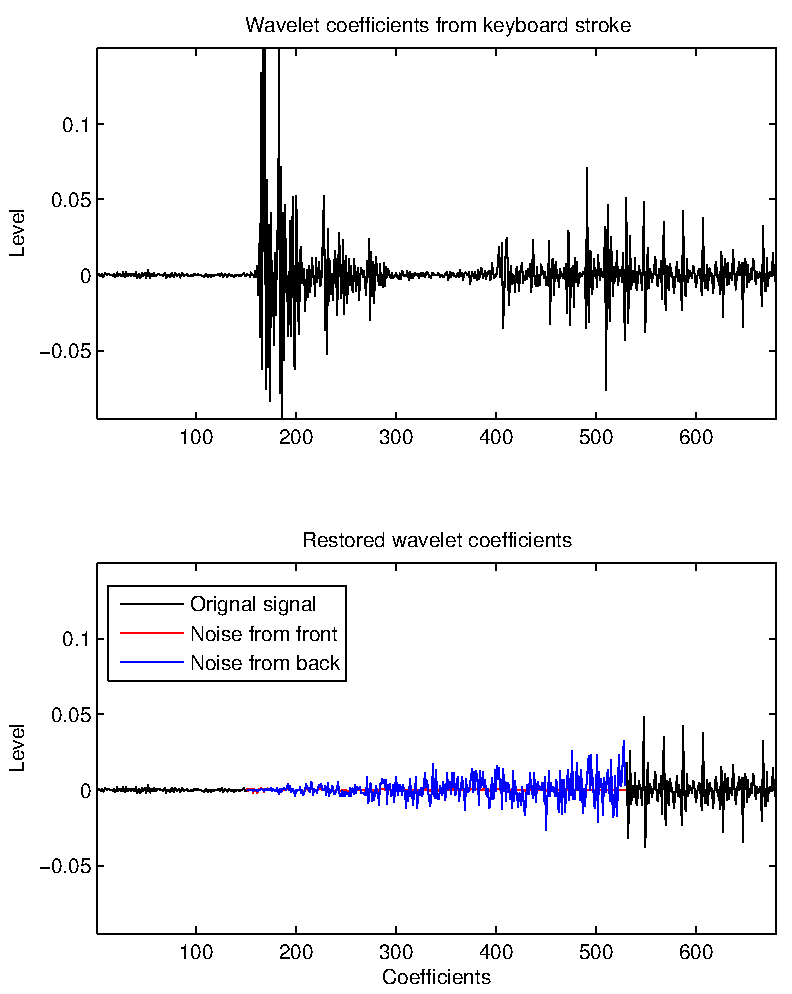
\includegraphics[width=110mm]{ResultsNoiseInsertion.pdf}
\begin{picture}(0,0)
\put(-300,390){(a)}
\put(-300,180){(b)}
\end{picture}
\caption{Example of noise insertion algorithm. (a) Original corrupted signal, (b) Forward (red) and backward (blue) noise interpolation.}
\label{fig:ResultsNoiseInsertion.pdf}
\end{figure}

\subsection{Forwards and backwards FIR filtering}
%Model theory
A simple approach to restoration of short corrupted intervals is to replace the corrupted samples and filter the corrupted region with an FIR filter with parameters drawn from the segment immediately prior to $\boldsymbol{x}_{\boldsymbol{-(i)}a}$ and following $\boldsymbol{x}_{\boldsymbol{-(i)}b}$ (if available) the corruption.

Consider first the block of data samples $\boldsymbol{x}$ drawn from an AR process with parameters $\boldsymbol{a}$. Given a known estimate of the detection state $\boldsymbol{i}$, zero pad the corrupted samples.

\begin{equation}\label{eq:RestBasicModelFilterZeros}
\boldsymbol{x} = \left[ \boldsymbol{x}_{\boldsymbol{-(i)}a}\quad \left[0,\ldots,0\right] \quad\boldsymbol{x}_{\boldsymbol{-(i)}b} \right].
\end{equation}

The block of data $\boldsymbol{x}$ is then filtered using the AR parameters up until the end of the corrupted section,

\begin{equation}\label{eq:RestBasicModelFilterEQ}
\boldsymbol{\hat{x}}_f = \Sigma_p^P \boldsymbol{x}_{n-p}a_p.
\end{equation}

The output signal $\boldsymbol{\hat{x}}_f$ now contains a basic estimate of the corrupted section which will be called the forward filtered estimate. Reversing the order of the samples in $\boldsymbol{x}$ denoting it $\boldsymbol{x'}$ and applying the filtering step up to the end of the zeroed out corruption section gives an estimate for the backwards filtered estimate.

\begin{equation}\label{eq:RestBasicModelFilterEQR}
\boldsymbol{\hat{x}'}_b = \Sigma_p^P \boldsymbol{x'}_{n-p}a_p.
\end{equation}

The forward $\boldsymbol{\hat{x}}_f$ and backward $\boldsymbol{\hat{x}}_b$ filtered estimates can now, if both are available, be faded together to produce a combined estimate for the corrupted sequence $\boldsymbol{\hat{x}}$.

An example of a reconstructed section on can be seen in Figure~\ref{fig:ResultsFiltering.pdf}. It is noted that for this example the reconstruction is done on wavelet coefficients. Figure~\ref{fig:ResultsFiltering.pdf}(a) shows, as in Figure~\ref{fig:ResultsNoiseInsertion.pdf}, the original signal and Figure~\ref{fig:ResultsFiltering.pdf}(a) shows an example of the various parts of the reconstruction.

\begin{figure} %ResultsFiltering.pdf
\centering
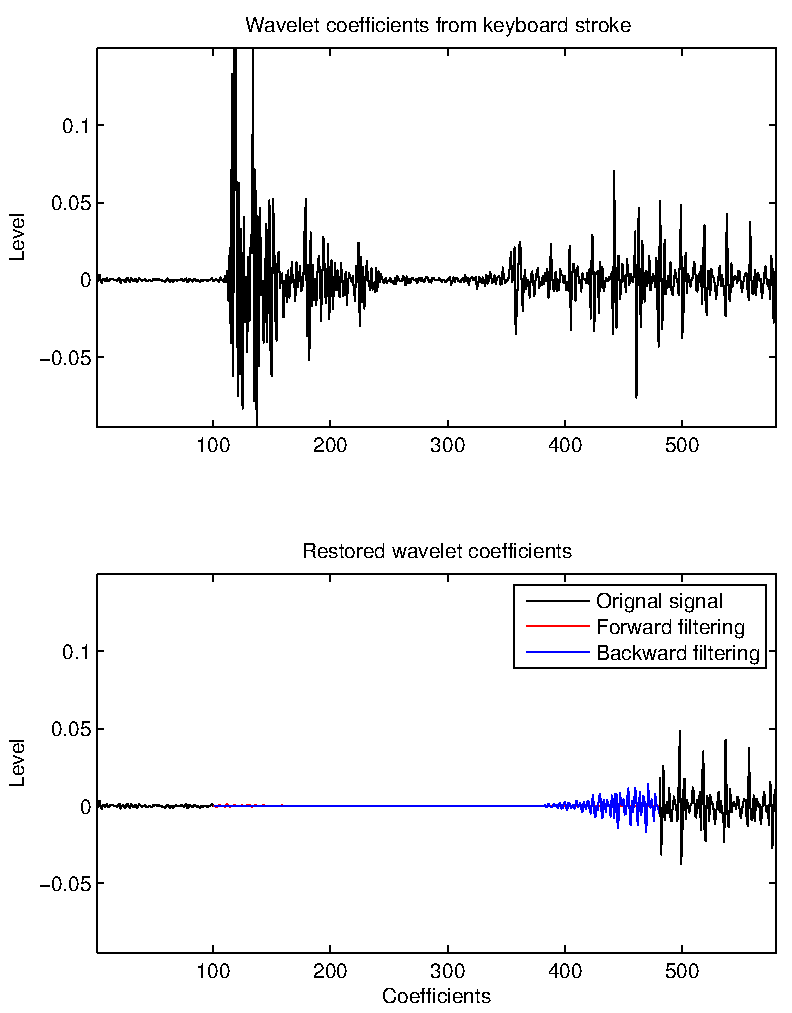
\includegraphics[width=110mm]{ResultsFiltering.pdf}
\begin{picture}(0,0)
\put(-300,390){(a)}
\put(-300,180){(b)}
\end{picture}
\caption{Example of forwards backwards algorithm. (a) Original corrupted signal, (b) Forward (red) and backward (blue) filtering interpolation.}
\label{fig:ResultsFiltering.pdf}
\end{figure}

\subsubsection{Filtering with noise}
It is possible to combine the noise insertion algorithm with the forward backward filtering algorithm to avoid a clearly audible dip in the loudness. This method proceeds as the original noise insertion method after which the forward backward filtering step is performed without zeroing the corrupted region.

Figure~\ref{fig:ResultsNoiseInsertionFiltering.pdf} shows an example of the noise insertion and filtering method applied to the same restoration example as in Figure~\ref{fig:ResultsNoiseInsertion.pdf} and \ref{fig:ResultsFiltering.pdf}.

\begin{figure} %ResultsNoiseInsertionFiltering.pdf
\centering
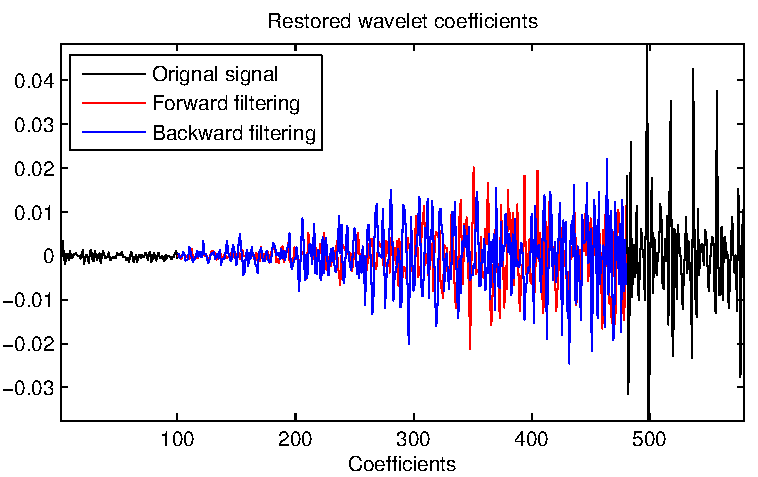
\includegraphics[width=110mm]{ResultsNoiseInsertionFiltering.pdf}
\begin{picture}(0,0)
\end{picture}
\caption{Example of forwards backwards algorithm.}
\label{fig:ResultsNoiseInsertionFiltering.pdf}
\end{figure}

\subsection{Burst scaling}
A different restoration approach can be derived from the noise burst detection method proposed in section~\ref{sec:WPdetectionNB}.
Based on the separation of the original data sequence in Equation~\ref{eq:modelgeneral} it was assumed that the majority of the transient information will be located in the residual, or non-tonal component. Considering the detection methods employed on the residual component, the restoration process could be done in either the time or the wavelet domain $w(n)$.

A Bayesian approach proceeds by estimating $p(\boldsymbol{v}_n | \boldsymbol{w}_n, i_n)$. Using Bayes' rule we get that

\begin{equation}\label{eq:BayesInterp}
p(\boldsymbol{v}_n | \boldsymbol{w}_n, i_n) \propto p(\boldsymbol{w}_n | \boldsymbol{v}_n , i_n) p(\boldsymbol{v}_n | i_n),
\end{equation}
where
\begin{equation}\label{eq:w|vi}
p(\boldsymbol{w}_n | \boldsymbol{v}_n, i_n = 1) = \mathcal{N}(\boldsymbol{v}_n, \Lambda),
\end{equation}
and
\begin{equation}\label{eq:v2}
p(\boldsymbol{v}_n | i_n) = p(\boldsymbol{v}_n) = \mathcal{N}(0, C_v).
\end{equation}
Substituting equation (\ref{eq:w|vi}) and (\ref{eq:v2}) into equation (\ref{eq:BayesInterp}) where the product is proportional to a third Gaussian,
\begin{equation}\label{eq:vwi}
p(v_n | \boldsymbol{w}_n, i_n = 1) \propto \mathcal{N}\left({(C_v + \Lambda)^{-1} C_v\boldsymbol{w}_n}, (C_v^{-1} + \Lambda^{-1})^{-1}\right)
\end{equation}

%\frac{\boldsymbol{w}_n}{\Lambda}\right).
In this case where both the background noise $v_n$ and the noise burst $\theta_n$ are Gaussian, estimating the mean of the conditional distribution equates to simply scaling corrupted samples by a factor of $({C_v + \Lambda})^{-1}{C_v}$ in a Wiener-style wavelet shrinkage (note the simple form of this in our case with diagonal covariance matrices).

An example of the burst scaling algorithm is seen in Figure~\ref{fig:ResultsScaled.pdf}. The reference variance for the wavelet coefficient sets $C_v$ is taken over a 5 second sequence. The pulse variance $\Lambda$ is a trained value which might vary from session to session, but for the restoration stage here the first 150 samples of the detected impulse is used.

\begin{figure} %ResultsScaled.pdf
\centering
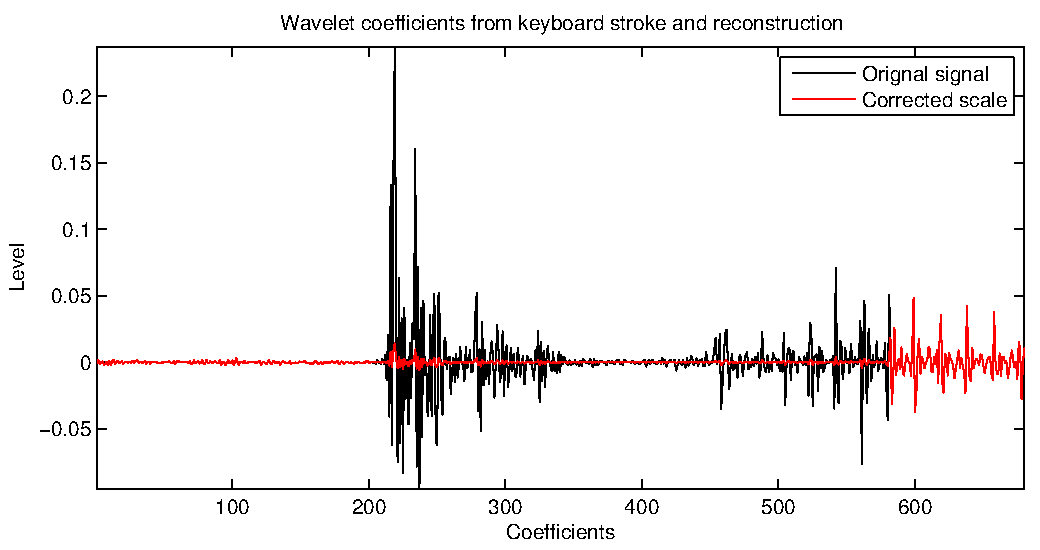
\includegraphics[width=100mm]{ResultsScaled.pdf}
\begin{picture}(0,0)
%\put(-245,235){Restored Example}
%\put(-200,0){Time}
\end{picture}
\caption{Examples of the burst scaling algorithm restoring corrupted wavelet coefficients.}
\label{fig:ResultsScaled.pdf}
\end{figure}

%While assuming corruptions as noise bursts works well for detection, it was found that a more pleasing restoration was achieved by simply inserting white noise bursts with background variance in the corrupted regions. Figure~\ref{fig:compareRecon} shows an example of the restoration on the example result from Figure~\ref{fig:Separation_Residual_Example} An even simpler restoration approach could potentially entirely remove the offending coefficients and a more complicated approach attempt to fill in the corrupted coefficients with an AR process trained on preceding and succeeding coefficients. Having estimated the most likely state of $i_n$ it is sometimes necessary also to filter out any very low frequency components of the transient that were removed with the voiced speech. Figure~\ref{fig:compareRecon} shows an example of the restored signal with the corrupted regions filtered with a high pass filter with a cutoff frequency of 120 Hz.
%
%\begin{figure} %compareRecon.pdf
%\centering
%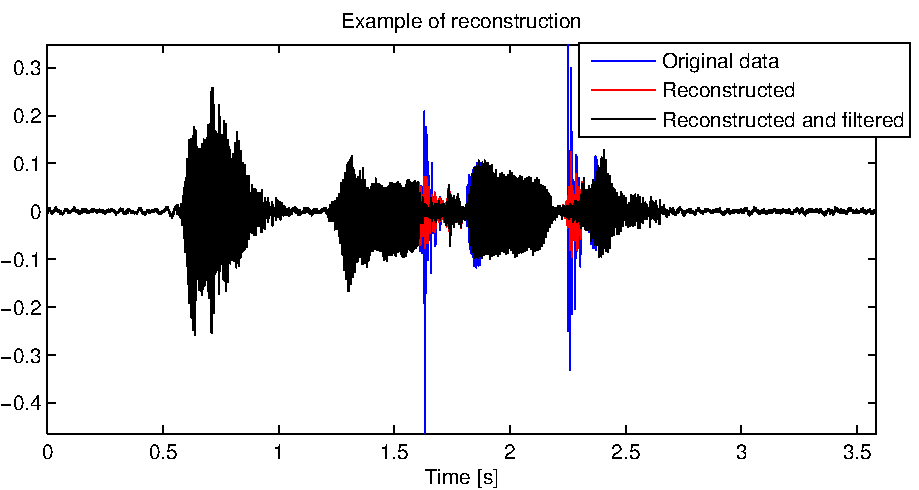
\includegraphics[width=100mm]{compareRecon.pdf}
%\begin{picture}(0,0)
%%\put(-245,235){Restored Example}
%%\put(-200,0){Time}
%\end{picture}
%\caption{Example of the algorithm interpolating corrupted waveform samples.}
%\label{fig:compareRecon}
%\end{figure}
%
%The final stage of the algorithm proceeds by recombining the processed residual with the keystrokes removed and the dictionary of tonal components from equation~\ref{eq:modelgeneral}.
%
%%Standard restoration, interpolation

\subsection{Least-Squares AR (LSAR)}\label{sec:ResidualRestorationLSAR}
For the restoration of samples in the residual component the Least Squares AR (LSAR) interpolator is considered here\cite{Godsill1998book}.

Assuming that the residual coefficients $\mathbf{x}$ are drawn from an AR process with parameters $\mathbf{a}$, and where

\begin{equation}\label{eq:LSAR0} \mathbf{A} =
\begin{bmatrix}
    -a_P    & \ldots & -a_1 & 1 & 0 & 0 & \ldots & 0 & 0 \\
    0       & -a_P & \ldots & -a_1 & 1 & 0 & 0 & \ldots & 0 \\
    \vdots  & \vdots    & \ddots & \ddots & \ddots & \ddots & \ddots & \vdots & \vdots \\
    \ldots  & 0 & 0 & -a_P    & \ldots & -a_1 & 1 & 0 & 0 \\
    0       & \ldots  & 0 & 0 & -a_P    & \ldots & -a_1 & 1 & 0 \\
    0       & 0 & \ldots  & 0 & 0 & -a_P    & \ldots & -a_1 & 1 \\
\end{bmatrix}.
\end{equation}

The excitation vector $\mathbf{e}$ can be expressed as

\begin{equation}\label{eq:LSAR1}
  \mathbf{e} = \mathbf{A}\mathbf{x},
\end{equation}

where $\mathbf{X}$, the data vector, can be reexpressed in terms of corrupted and uncorrupted, or known $\mathbf{K}$ and unknown $\mathbf{U}$), samples

\begin{align}\label{eq:LSAR2}
  \mathbf{e} = & \mathbf{A} (\mathbf{U}\mathbf{x}_{\mathbf{(i)}} + \mathbf{K}\mathbf{x}_{\mathbf{-(i)}}) \\
  \mathbf{e} = & \mathbf{A}_{\mathbf{(i)}} \mathbf{x}_{\mathbf{(i)}} + \mathbf{A}_{\mathbf{-(i)}}\mathbf{x}_{\mathbf{-(i)}}.
\end{align}

Now the sum squared prediction error can be calculated as

\begin{equation}\label{eq:LSAR3}
  E = \sum^N_{n=P+1} e^2_n = \mathbf{e}^T\mathbf{e}.
\end{equation}

The Least Squares (LS) interpolator is obtained as the interpolated data vector $\mathbf{x}_{\mathbf{(i)}}$ which minimises the error in equation~\ref{eq:LSAR3}:

\begin{equation}\label{eq:LSAR4}
  \mathbf{x}^{\mathrm{LS}}_{\mathbf{(i)}} = \argmin{\mathbf{x}_{\mathbf{(i)}}} \{ E \}.
\end{equation}

$E$ can expanded and differentiated to find its minimum:

\begin{align}\label{eq:LSAR5}
  E = & \mathbf{e}^T\mathbf{e} \\
  \frac{\partial E}{\partial \mathbf{x}_{\mathbf{(i)}}} = & 2\mathbf{e}^T \frac{\partial \mathbf{e}}{\partial \mathbf{x}_{\mathbf{(i)}}} \\
   = & 2 (\mathbf{A}_{\mathbf{(i)}} \mathbf{x}_{\mathbf{(i)}} + \mathbf{A}_{\mathbf{-(i)}}\mathbf{x}_{\mathbf{-(i)}})^T \mathbf{A}_{\mathbf{(i)}} = 0
\end{align}

Solving for $\mathbf{x}_{\mathbf{(i)}}$ we have that:

\begin{equation}\label{eq:LSAR6}
  \mathbf{x}^{\mathrm{LS}}_{\mathbf{(i)}} = - (\mathbf{A}_{\mathbf{(i)}}^T \mathbf{A}_{\mathbf{(i)}} )^{-1}\mathbf{A}_{\mathbf{(i)}}^T\mathbf{A}_{\mathbf{-(i)}}\mathbf{x}_{\mathbf{-(i)}}
\end{equation}

An example of the LSAR interpolation algorithm is shown in Figure~\ref{fig:RestoredLSARExample}(a) and \ref{fig:RestoredLSARExample2}(b), where 2 different sets of Wavelet coefficients have had an impulse detection restored. Both examples are of audio sampled at 16kHz and coefficients are from a Wavelet decomposition done to the third level. Figure~\ref{fig:RestoredLSARExample}(a) uses the same detection example as the previous examples while  Figure~\ref{fig:RestoredLSARExample2}(b) shows a restoration example, from the same audio sequence, which showcases more of the algorithms restoration abilities.

\begin{figure}
\begin{minipage}[b]{1.0\linewidth}
  \centering
  \centerline{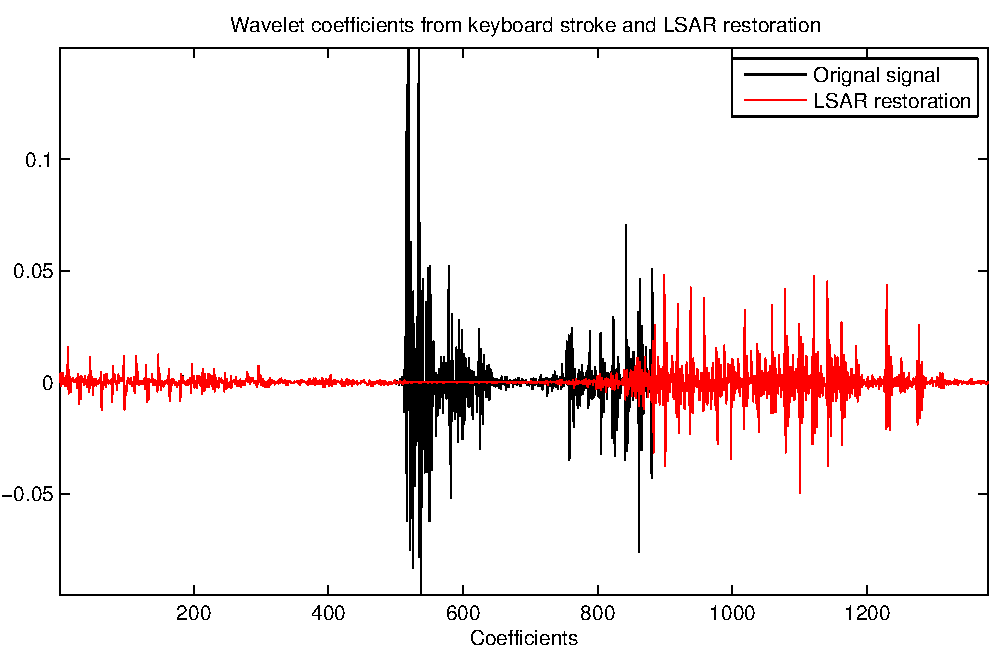
\includegraphics[width=10cm]{RestoredLSARExample1.pdf}}
%  \vspace{2.0cm}
  %\centerline{(a)}\medskip
\end{minipage}
\begin{minipage}[b]{1.0\linewidth}
  \centering
  \centerline{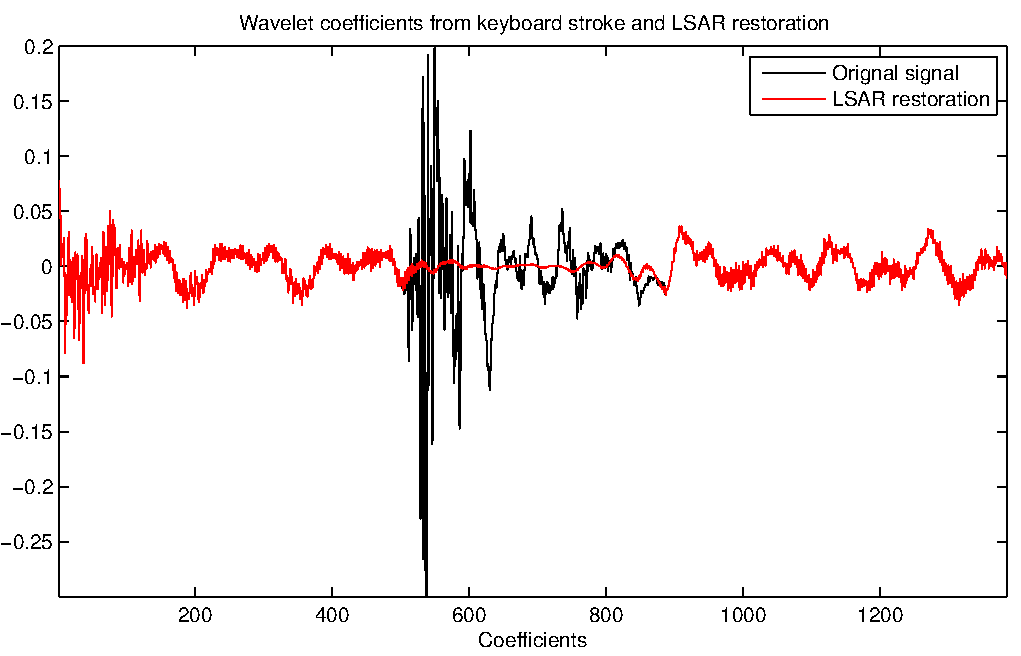
\includegraphics[width=10cm]{RestoredLSARExample2.pdf}}
  \begin{picture}(0,0)
\put(-120,382){a)}
\put(-120,195){b)}
\end{picture}
%  \vspace{1.5cm}
  %\centerline{(b)}\medskip
\end{minipage}
\caption{Examples of the LSAR algorithm interpolating corrupted wavelet coefficients.}
\label{fig:RestoredLSARExample}
\end{figure}

%\begin{figure}% %Restore_LSAR_1.pdf
%\centering
%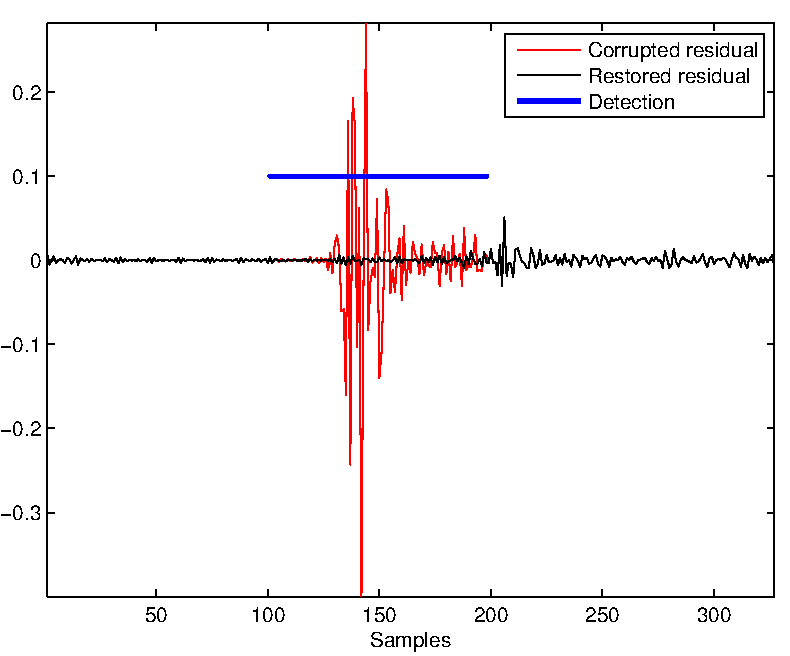
\includegraphics[width=100mm]{Restore_LSAR_1.pdf}
%\begin{picture}(0,0)
%\put(-245,235){Restored Wavelet coefficients Example 1}
%%\put(-200,0){Time}
%\end{picture}
%\caption{Example of the LSAR algorithm interpolating 85 missing Wavelet coefficients at level 3.}
%\label{fig:Restore_LSAR_1.pdf}
%\end{figure}
%
%\begin{figure} %Restore_LSAR_2.pdf
%\centering
%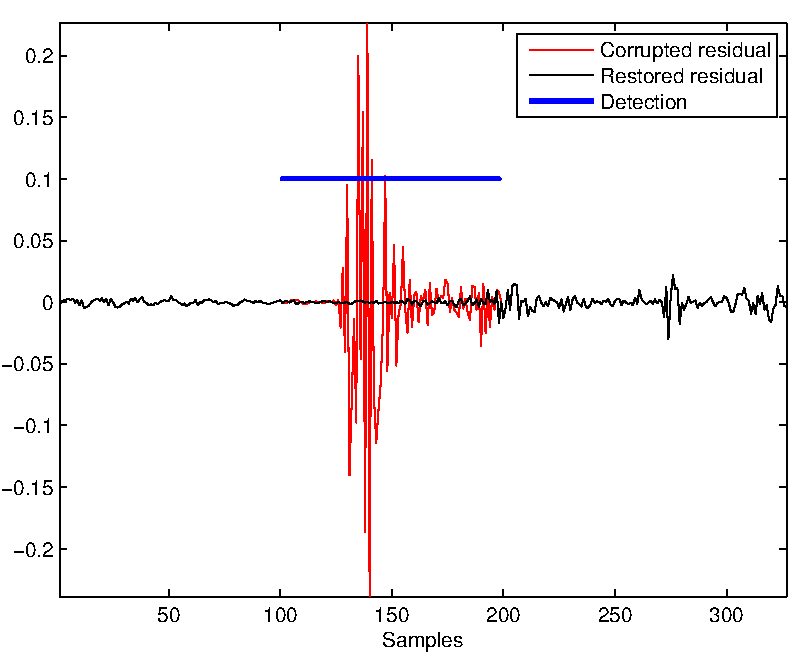
\includegraphics[width=100mm]{Restore_LSAR_2.pdf}
%\begin{picture}(0,0)
%\put(-245,235){Restored Wavelet coefficients Example 2}
%%\put(-200,0){Time}
%\end{picture}
%\caption{Example of the LSAR algorithm interpolating 85 missing Wavelet coefficients at level 3.}
%\label{fig:Restore_LSAR_2.pdf}
%\end{figure}

\section{Tonal Restoration}
While the aim of the pre processing separation stage is to separate out tonal components from transient noise events, the tonal components themselves occasionally retain components introduced by the noise events. These tonal noise components are not always present, but factors such as the amplitude of the impulse, mechanical properties of the keyboard or the laptop enclosure and even the surface on which the keyboard or computer is placed can have an impact on whether or not these components are present to the extent that get identified as tonal components. Constraints such as frame sizes in the system can also add to the amount of noise leaking through to the tonal components. A short frame size can contribute to this effect.

\subsection{Basic filtering}\label{sec:TonalFiltering}
The most common noise component left in the tonal component of the signal is a low frequency \emph{bump}. Figure~\ref{fig:TonalArtefactSpectrumExample.png} shows an example of this, with an accompanying spectrogram. While it may be difficult to clearly visualise the extent of the corruption within a speech segment, it is although clearly audible.\footnote{\sound{Tonal\_Example.wav}}

\begin{figure} %TonalArtefactSpectrumExample.png
\centering
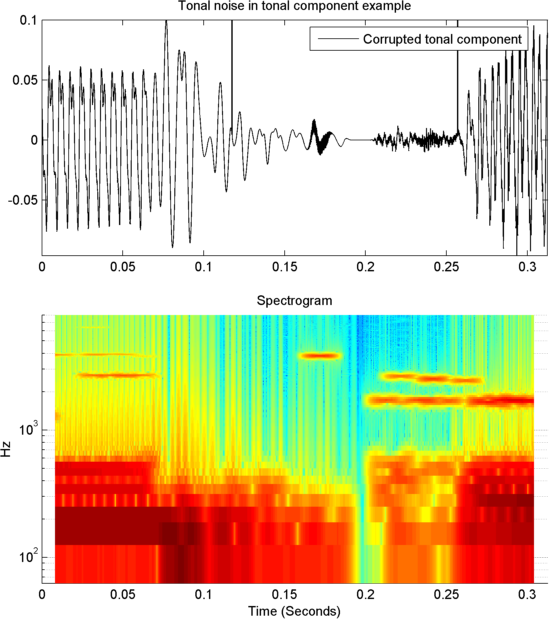
\includegraphics[width=120mm]{TonalArtefactSpectrumExample.png}
\begin{picture}(0,0)
%\put(-320,442){a)}
%\put(-320,290){b)}
%\put(-320,140){c)}
\end{picture}
\caption{Example of low frequency tonal noise. A \emph{bump}. Top: Waveform and Bottom: Spectrogram of same sequence.}
\label{fig:TonalArtefactSpectrumExample.png}
\end{figure}

A simple approach to removing low frequency noise is to apply standard high pass filter to the corrupted region. Fading in and out from this filtered segment will remove the effect of discontinuities. Figure~\ref{fig:TonalFilteringExample.pdf} shows the same example of a tonal noise component as in Figure~\ref{fig:TonalArtefactSpectrumExample.png} and the process for removing it. In Figure~\ref{fig:TonalFilteringExample.pdf}(a) the original corrupted signal can be seen together with a plot of the detection state. The unrestored tonal component is seen in Figure~\ref{fig:TonalFilteringExample.pdf}(c) with a mixing indicator showing the state of the mixing process which tapers the amplitude from 100\% to 0\% in 200 samples or an $1/80$ of a second at the sampling rate of 16000 Hz. Figure~\ref{fig:TonalFilteringExample.pdf}(b) shows the inverse mixing indicator and the high pass filtered signal with a cutoff frequency of 120 Hz.

\begin{figure} %TonalFilteringExample.pdf
\centering
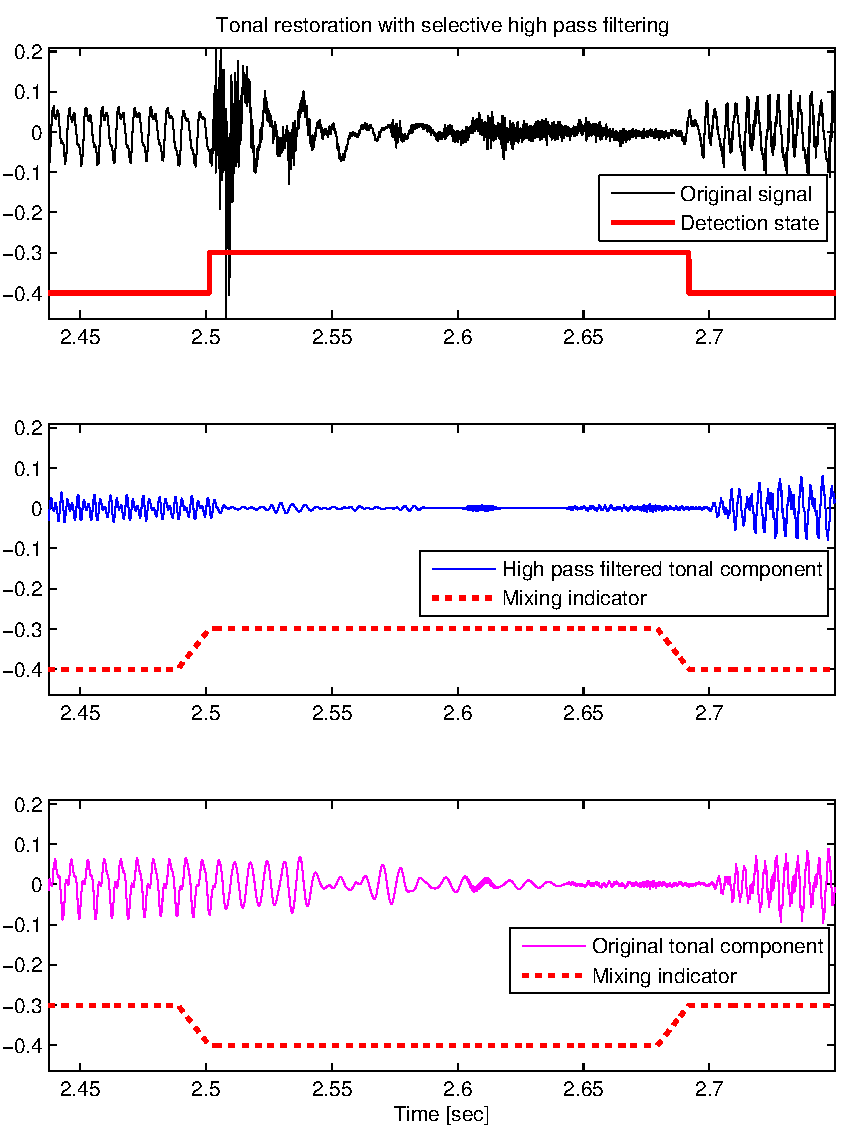
\includegraphics[width=120mm]{TonalFilteringExample.pdf}
\begin{picture}(0,0)
\put(-320,442){a)}
\put(-320,290){b)}
\put(-320,140){c)}
\end{picture}
\caption{Example of simple tonal restoration using filtering. a) Original complete signal and detection state, b) High pass filtered (200Hz) tonal component with mixing indicator, and c) original tonal component with mixing indicator.}
\label{fig:TonalFilteringExample.pdf}
\end{figure}

The result of the simple tonal filtering example can be seen in Figure~\ref{fig:TonalArtefactSpectrumExampleFiltered.png}.

\begin{figure} %TonalArtefactSpectrumExampleFiltered.png
\centering
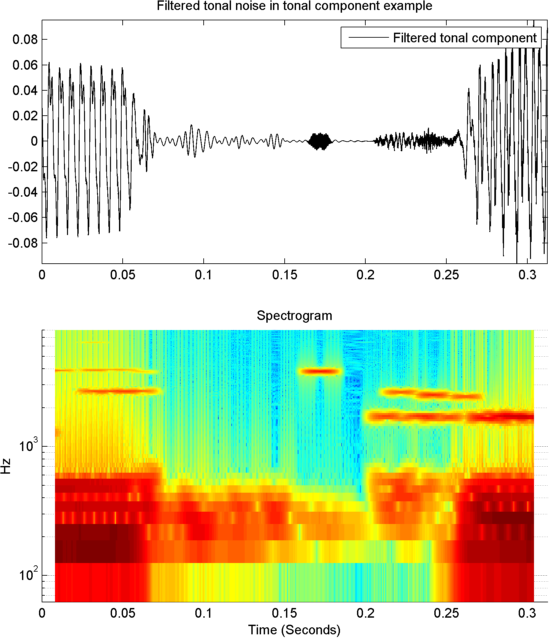
\includegraphics[width=120mm]{TonalArtefactSpectrumExampleFiltered.png}
\begin{picture}(0,0)
%\put(-320,442){a)}
%\put(-320,290){b)}
%\put(-320,140){c)}
\end{picture}
\caption{Example of simple tonal restoration using filtering.}
\label{fig:TonalArtefactSpectrumExampleFiltered.png}
\end{figure}

\subsection{Historic filtering}
%- Historic Frequency logic and filtering (amplitudes)
%- Future restoration (fading)
While the separation algorithm works by modeling the speech as distinctive tonal components some keystroke noise pulses also exhibit strong tonal components beyond those seen in section~\ref{sec:TonalFiltering}. As mentioned previously, this may be due to a range of physical conditions but possibly also due to constraints on the frame size in a system. In this section a frame size of 10 ms is assumed. While the results from the simple high pass filtering algorithm presented in section~\ref{sec:TonalFiltering} does manage to remove low frequency tonal noise \emph{bumps} in the audio it fails to remove higher frequency tonal components. This section will focus on a generalised approach to removing tonal noise components introduced by some keyboard strokes, and will specifically focus on doing this in a sequential frame based and computationally simple manner.

Figure~\ref{fig:TonalRestoration_Spec_Orig.png} shows the spectrogram of a keyboard noise pulse embedded in a voiced audio segment. The method described here will be applied to this audio example and followed throughout this section.

\begin{figure} %TonalRestoration_Spec_Orig.png
\centering
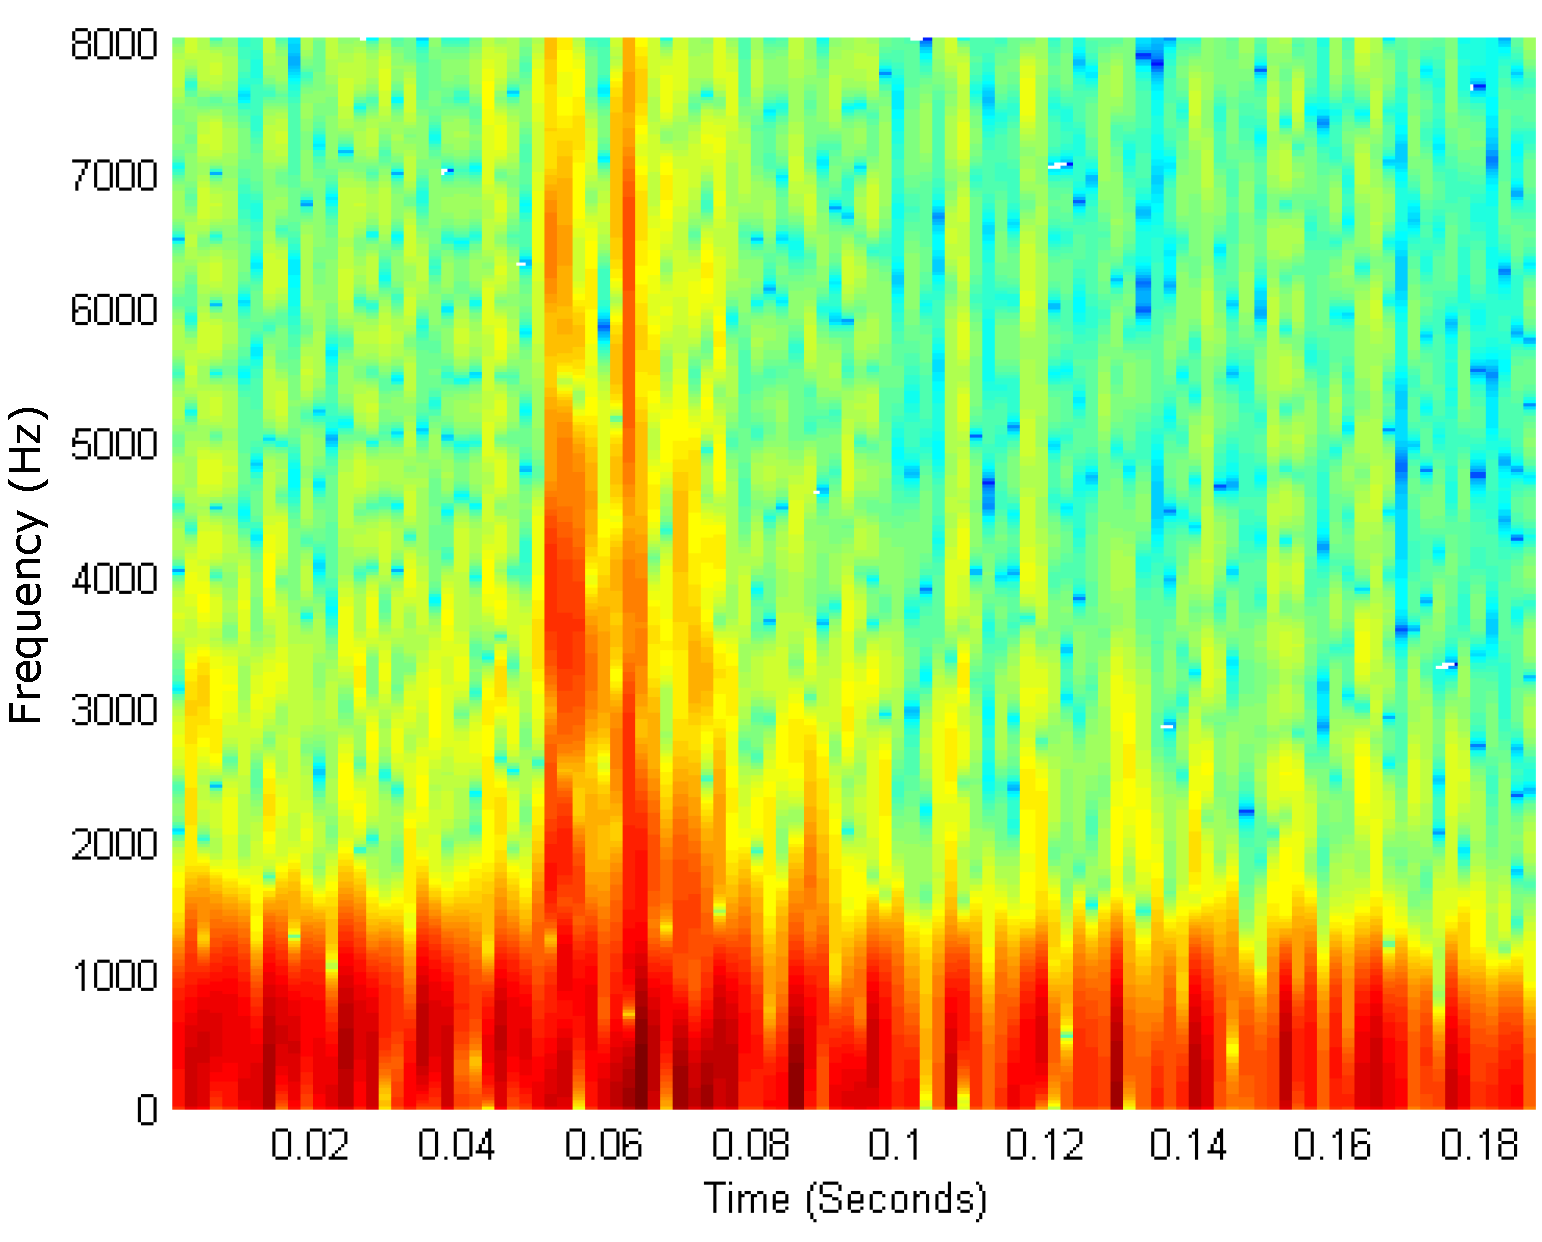
\includegraphics[width=100mm]{TonalRestoration_Spec_Orig.png}
\begin{picture}(0,0)
\put(-200,235){Spectrum of original signal}
%\put(-200,0){Time}
\end{picture}
\caption{Example of corrupted audio segment.}
\label{fig:TonalRestoration_Spec_Orig.png}
\end{figure}

Figure~\ref{fig:TonalRestoration_Spec_ResidualRestoration.png} shows a spectrogram of the audio segment from Figure~\ref{fig:TonalRestoration_Spec_Orig.png} with the LSAR residual restoration from section~\ref{sec:ResidualRestorationLSAR} applied. The separation algorithm has largely kept the voiced signal below 1500 Hz intact but some higher frequency information from the noise pulse has also been detected as tonal components and hence are still clearly visible in the spectrogram. These components, combined with the underlying voiced signal, is what can sometimes be seen detected as tonal components by the separation algorithm. Rather that replacing the data from the influenced buffers completely, like was done for the majority of the residual restoration algorithms, this sections will explore a heuristic method for filtering out interfering tonal components while keeping voiced components intact and undisturbed.

\begin{figure} %TonalRestoration_Spec_ResidualRestoration.png
\centering
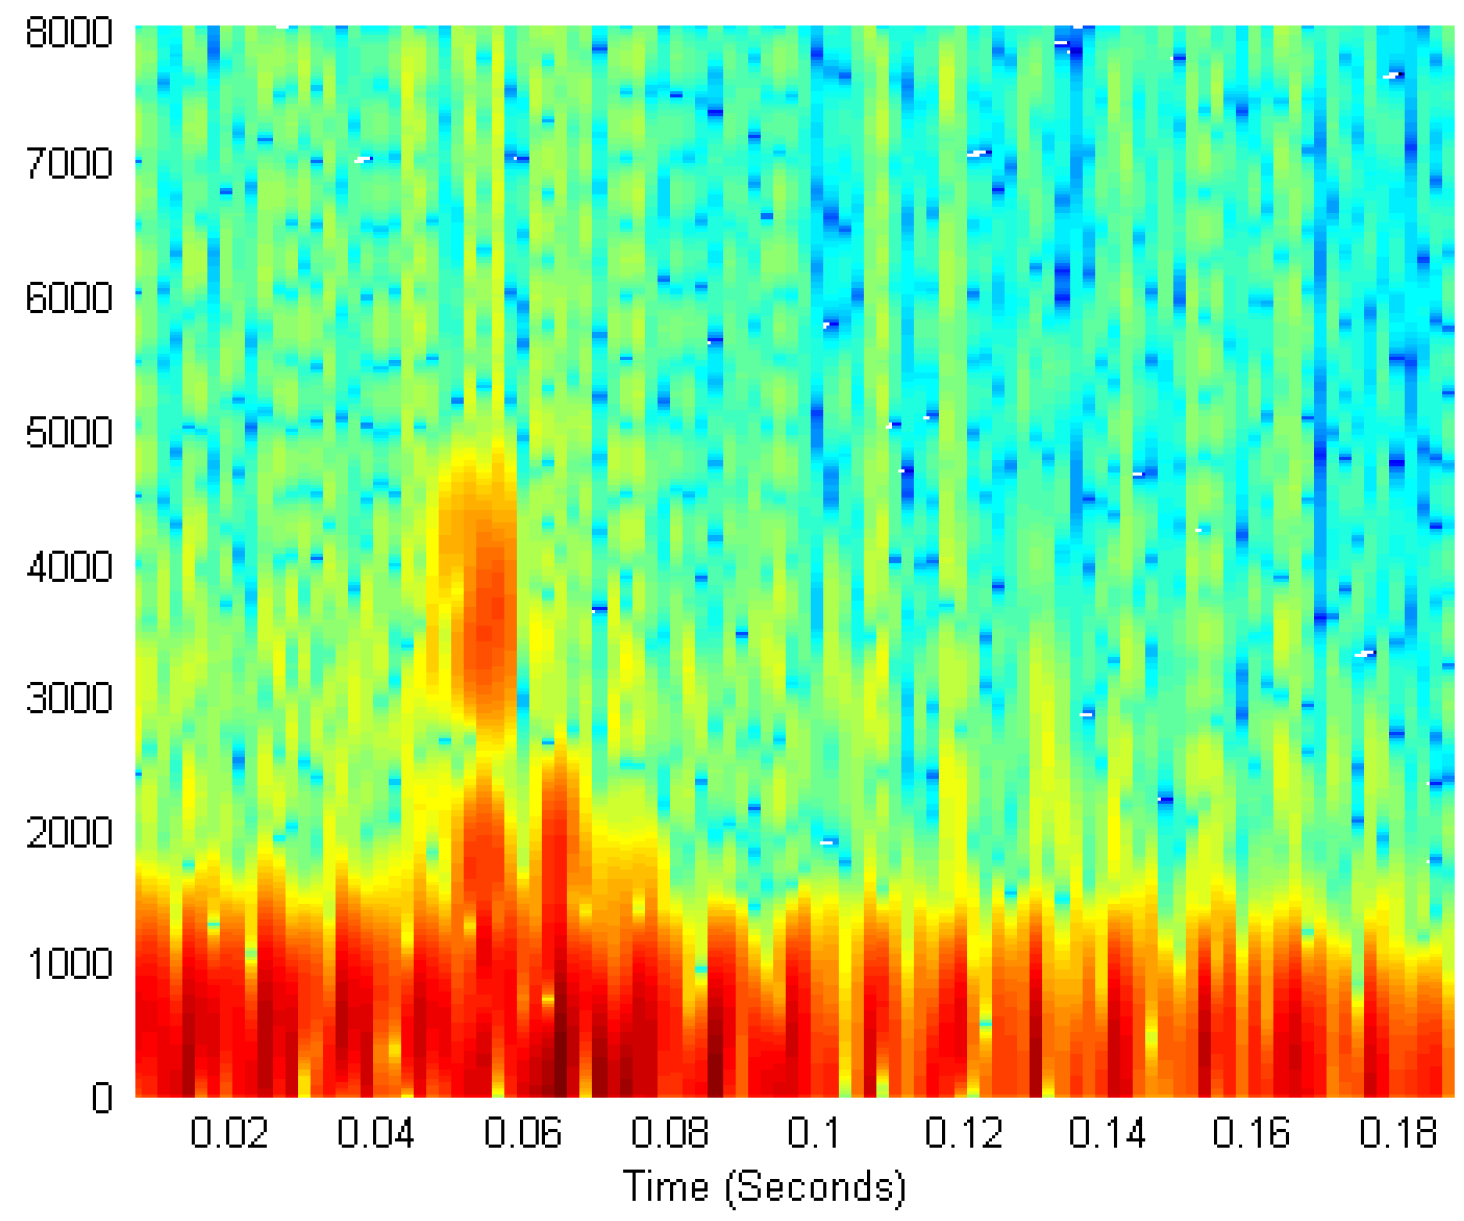
\includegraphics[width=100mm]{TonalRestoration_Spec_ResidualRestoration.png}
\begin{picture}(0,0)
\put(-245,235){Spectrogram of signal after residual restoration}
%\put(-200,0){Time}
\end{picture}
\caption{Example of residual restored audio segment}
\label{fig:TonalRestoration_Spec_ResidualRestoration.png}
\end{figure}

Since voiced components of speech generally are seen for at least 100 ms, this tonal restoration algorithm starts by keeping a record of active tonal atoms. These are already computed through the separation algorithm and so this only requires additional memory while running. Figure~\ref{fig:TonalRestoration_Spec_ResidualRestorationFrames.png} shows a grid of 10 ms frames overlayed on the previous audio frames. The grid in Figure~\ref{fig:TonalRestoration_Spec_ResidualRestorationFrames.png} indicates the extent of historic buffer and the data stored will be the tonal components that are selected by the separation algorithm as well as the magnitude of these frequencies within the buffers.

\begin{figure} %TonalRestoration_Spec_ResidualRestorationFrames.png
\centering
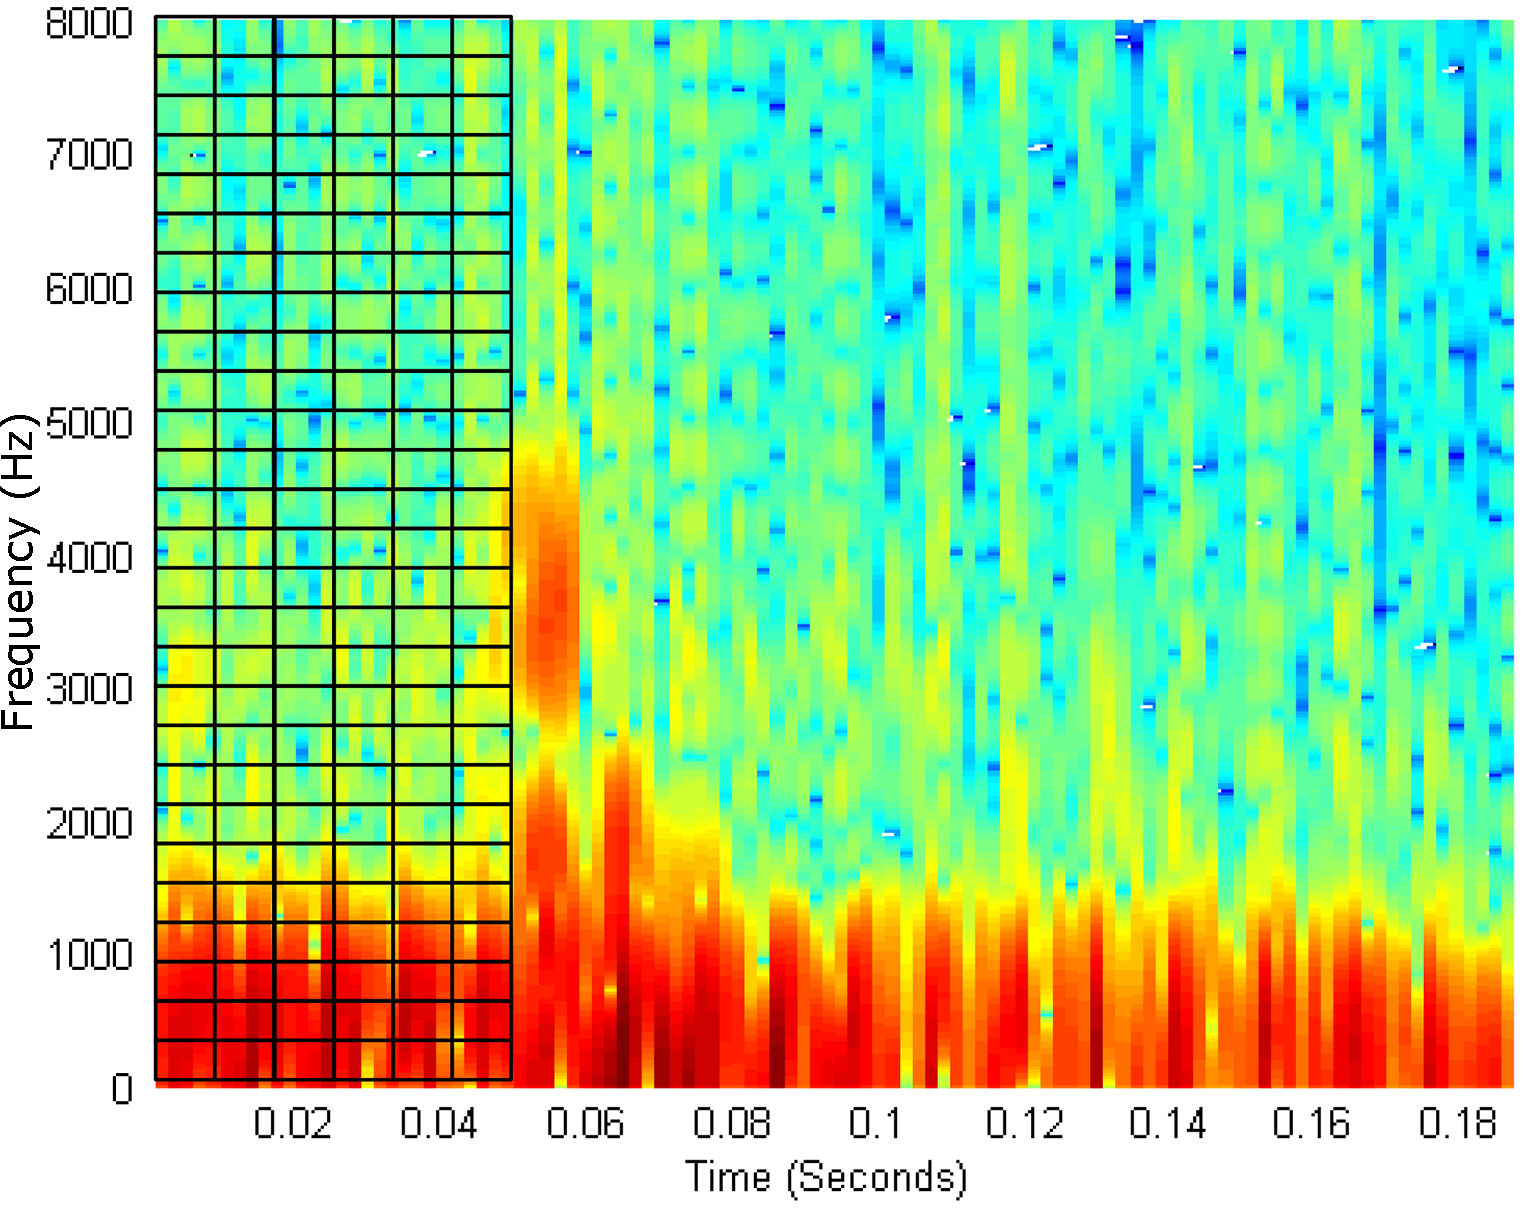
\includegraphics[width=100mm]{TonalRestoration_Spec_ResidualRestorationFrames.png}
\begin{picture}(0,0)
\put(-250,235){Spectrogram of signal after residual restoration}
%\put(-200,0){Time}
\end{picture}
\caption{Example of tonal filtering algorithm of the data from Figure~\ref{fig:TonalRestoration_Spec_Orig.png}}
\label{fig:TonalRestoration_Spec_ResidualRestorationFrames.png}
\end{figure}

Figure~\ref{fig:TonalRestoratio_FramesLogic.pdf} shows a diagram of the logic in the tonal filtering algorithm applied to the tonal component of a frame or buffer that is found to be corrupted by a noise pulse. The algorithm proceed by calculating the binary sum vector from the magnitude history buffer. This vector will serve as a template for which frequencies would be expected in a corrupted frame. The vector in Figure~\ref{fig:TonalRestoratio_FramesLogic.pdf} annotated as ``Noise profile'' indicates tonal components detected during the corrupted frame. Filtering the current noise profile based on the magnitude history it is now possible to remove newly introduced frequencies that likely are due to the corruption.

\begin{figure} %TonalRestoratio_FramesLogic.pdf
\centering
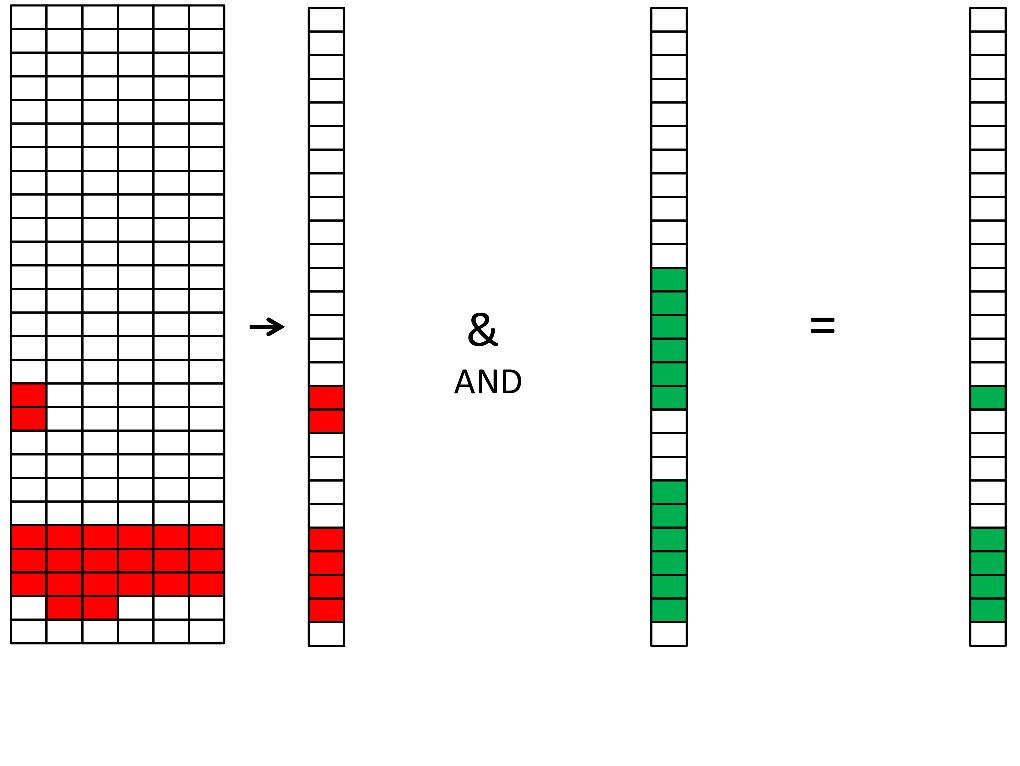
\includegraphics[width=120mm]{TonalRestoratio_FramesLogic.pdf}
\begin{picture}(0,0)
\put(-260,265){Tonal filtering algorithm diagram}
\put(-340,25){Magnitude}
\put(-340,10){history}

\put(-240,25){Binary}
\put(-240,10){sum}

\put(-130,25){Noise}
\put(-130,10){profile}

\put(-25,25){Filtered}
\put(-25,10){noise frame}
\end{picture}
\caption{Example of part of the tonal restoration algorithm.}
\label{fig:TonalRestoratio_FramesLogic.pdf}
\end{figure}

While the filtered tonal components in a corrupted frame might now contain only plausibly correct tonal components these might still be of a significantly higher magnitude that seen in the previous uncorrupted voiced speech frames. Figure~\ref{fig:TonalRestoratio_FramesLogic2.pdf} shows a diagram of how the tonal restoration algorithm proceeds by scaling the filtered tonal components to a plausible magnitude. The median values from the historic magnitude buffer is computed and applied to the filtered tonal components.

\begin{figure} %TonalRestoratio_FramesLogic2.pdf
\centering
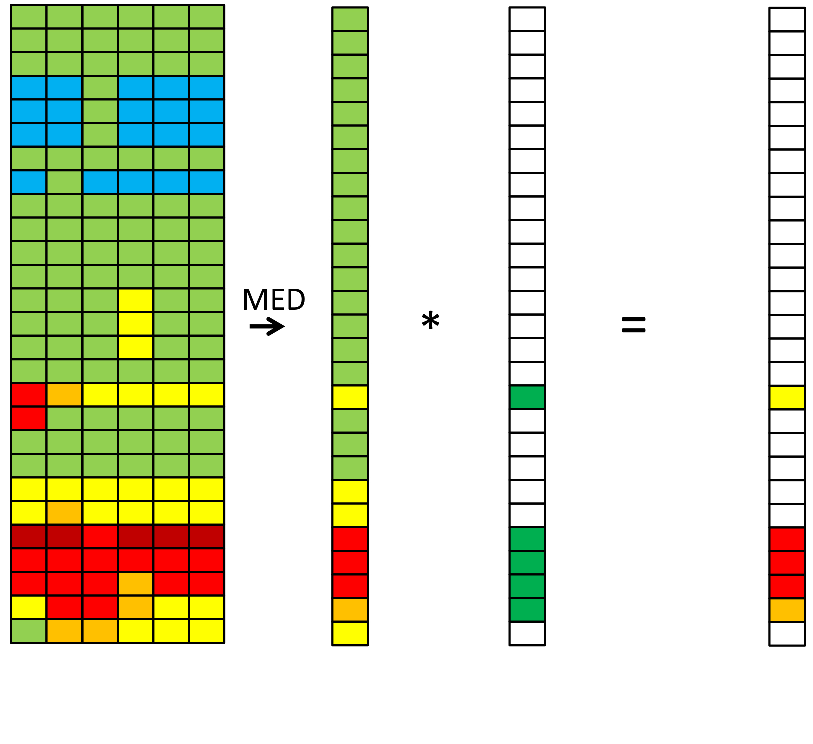
\includegraphics[width=100mm]{TonalRestoratio_FramesLogic2.pdf}
\begin{picture}(0,0)
\put(-250,265){Tonal scaling algorithm diagram}
\put(-280,20){Magnitude}
\put(-280,5){history}

\put(-180,20){Median}
\put(-180,5){values}

\put(-110,20){Filtered}
\put(-110,5){noise frame}

\put(-20,20){Filtered + scaled}
\put(-20,5){noise frame}
\end{picture}
\caption{Example of part of the tonal restoration algorithm.}
\label{fig:TonalRestoratio_FramesLogic2.pdf}
\end{figure}



\begin{figure} %TonalRestoratio_Spec_MagFiltScale.png
\centering
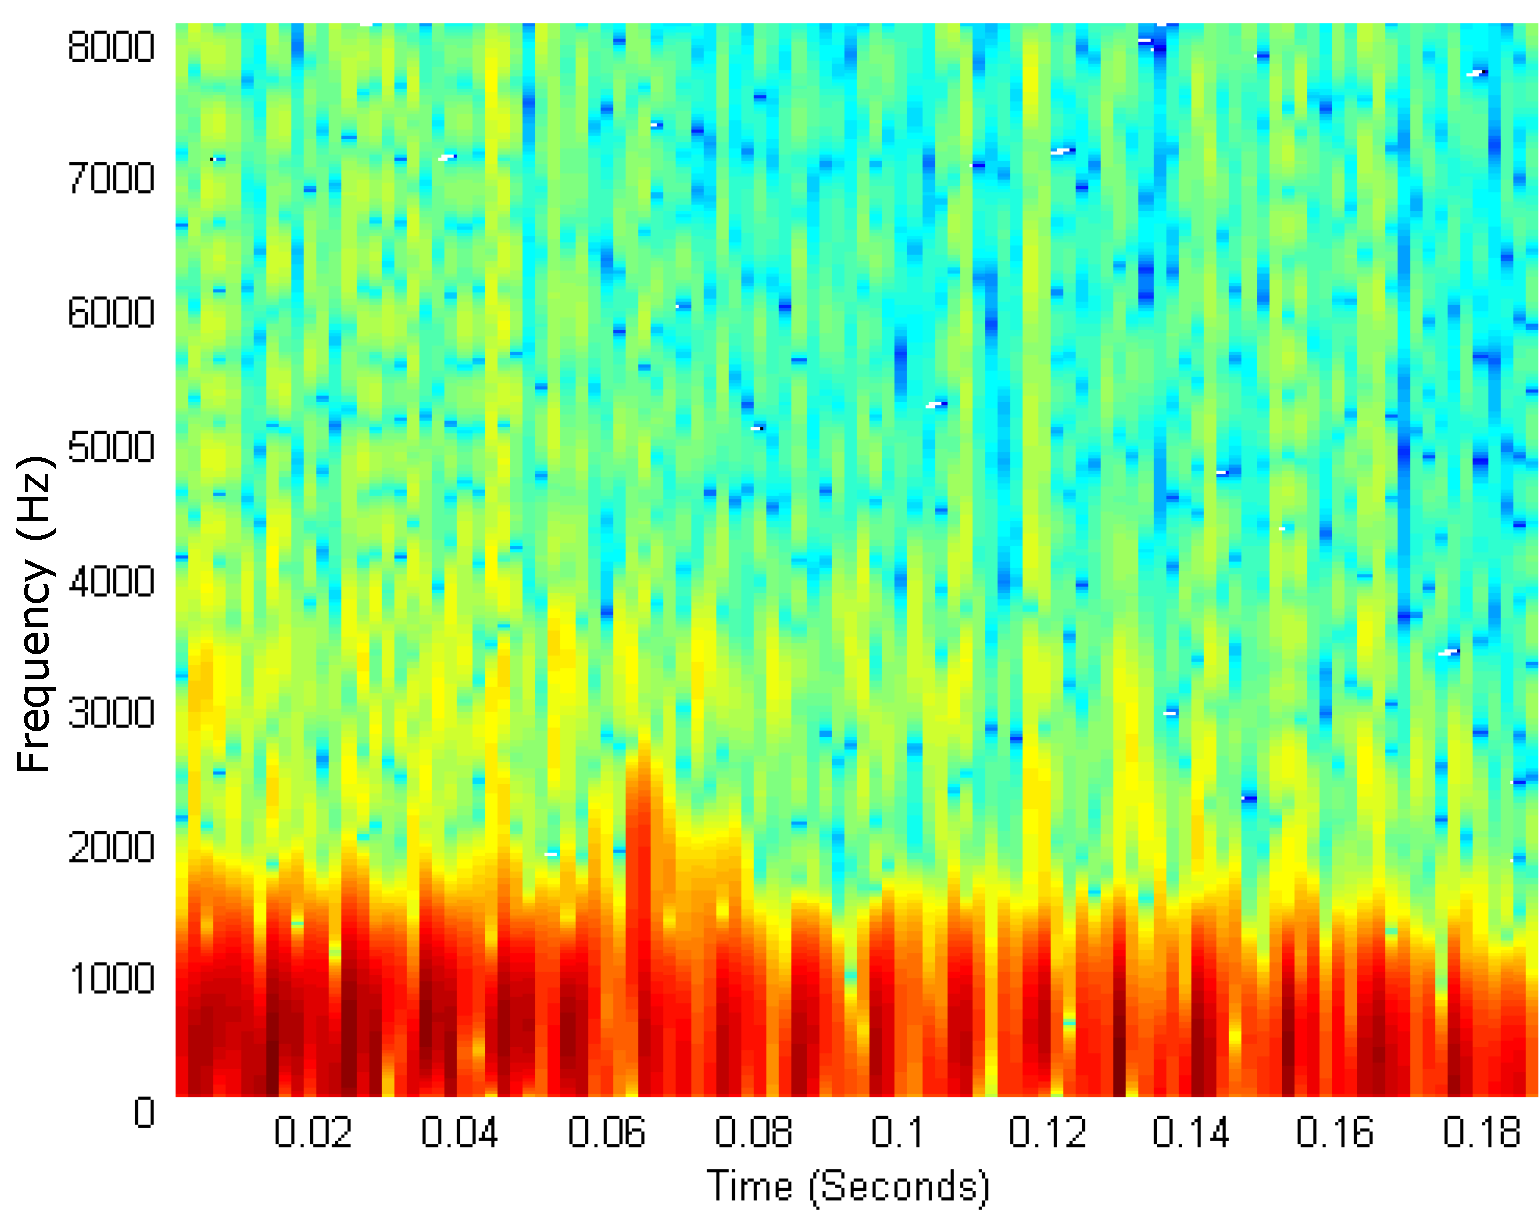
\includegraphics[width=100mm]{TonalRestoratio_Spec_MagFiltScale.png}
\begin{picture}(0,0)
\put(-250,235){Spectrum of signal after residual restoration}
\end{picture}
\caption{Example of residual restored and magnitude scaled audio segment}
\label{fig:TonalRestoratio_Spec_MagFiltScale.png}
\end{figure}

After applying both tonal filtering and rescaling Figure~\ref{fig:TonalRestoratio_Spec_MagFiltScale.png} shows the resulting spectrogram. While the initial pulse has been removed from the spectrogram a secondary pulse is still visible. This pulse shows how louder pulses will influence multiple buffers and hence it is necessary to employ filtering procedures for a number of frames after each detected corruption.

Figure~\ref{fig:TonalRestoratio_TonalFuture.pdf} shows a diagram of the logic employed to filter out remnants of noise pulses following a keyboard stroke detection. The algorithm contains 2 major components. First it applies a window function to the future tonal components so at the end of the procedure the algorithm performs as before a corruption was seen. Secondly the algorithm continues to apply the filtering and rescaling functions from the historic buffer. Since this second part of the algorithm is largely made up data this will be faded out as the real current data is faded back in.

\begin{figure} %TonalRestoratio_TonalFuture.pdf
\centering
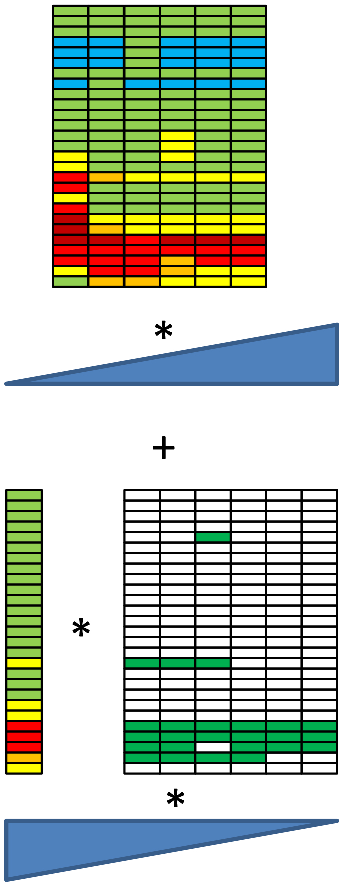
\includegraphics[width=70mm]{TonalRestoratio_TonalFuture.pdf}
\begin{picture}(0,0)
%top
\put(-200,525){Tonal restoration of future buffers}

%left side
\put(-260,150){Magnitude}
\put(-260,135){history}

%right side
\put(10,440){Tonal}
\put(10,425){future}

\put(10,310){Fade in}
\put(10,20){Fade out}

\put(10,150){Filtered}
\put(10,135){future tones}
\end{picture}
\caption{Example of tonal restoration algorithm following a corruption.}
\label{fig:TonalRestoratio_TonalFuture.pdf}
\end{figure}

The effect of this complete tonal restoration algorithm can be seen in Figure~\ref{fig:TonalRestoratio_Spec_FullRestoration.png}. The corruption has been completely removed and replaced with plausible looking data.

\begin{figure} %TonalRestoratio_Spec_FullRestoration.png
\centering
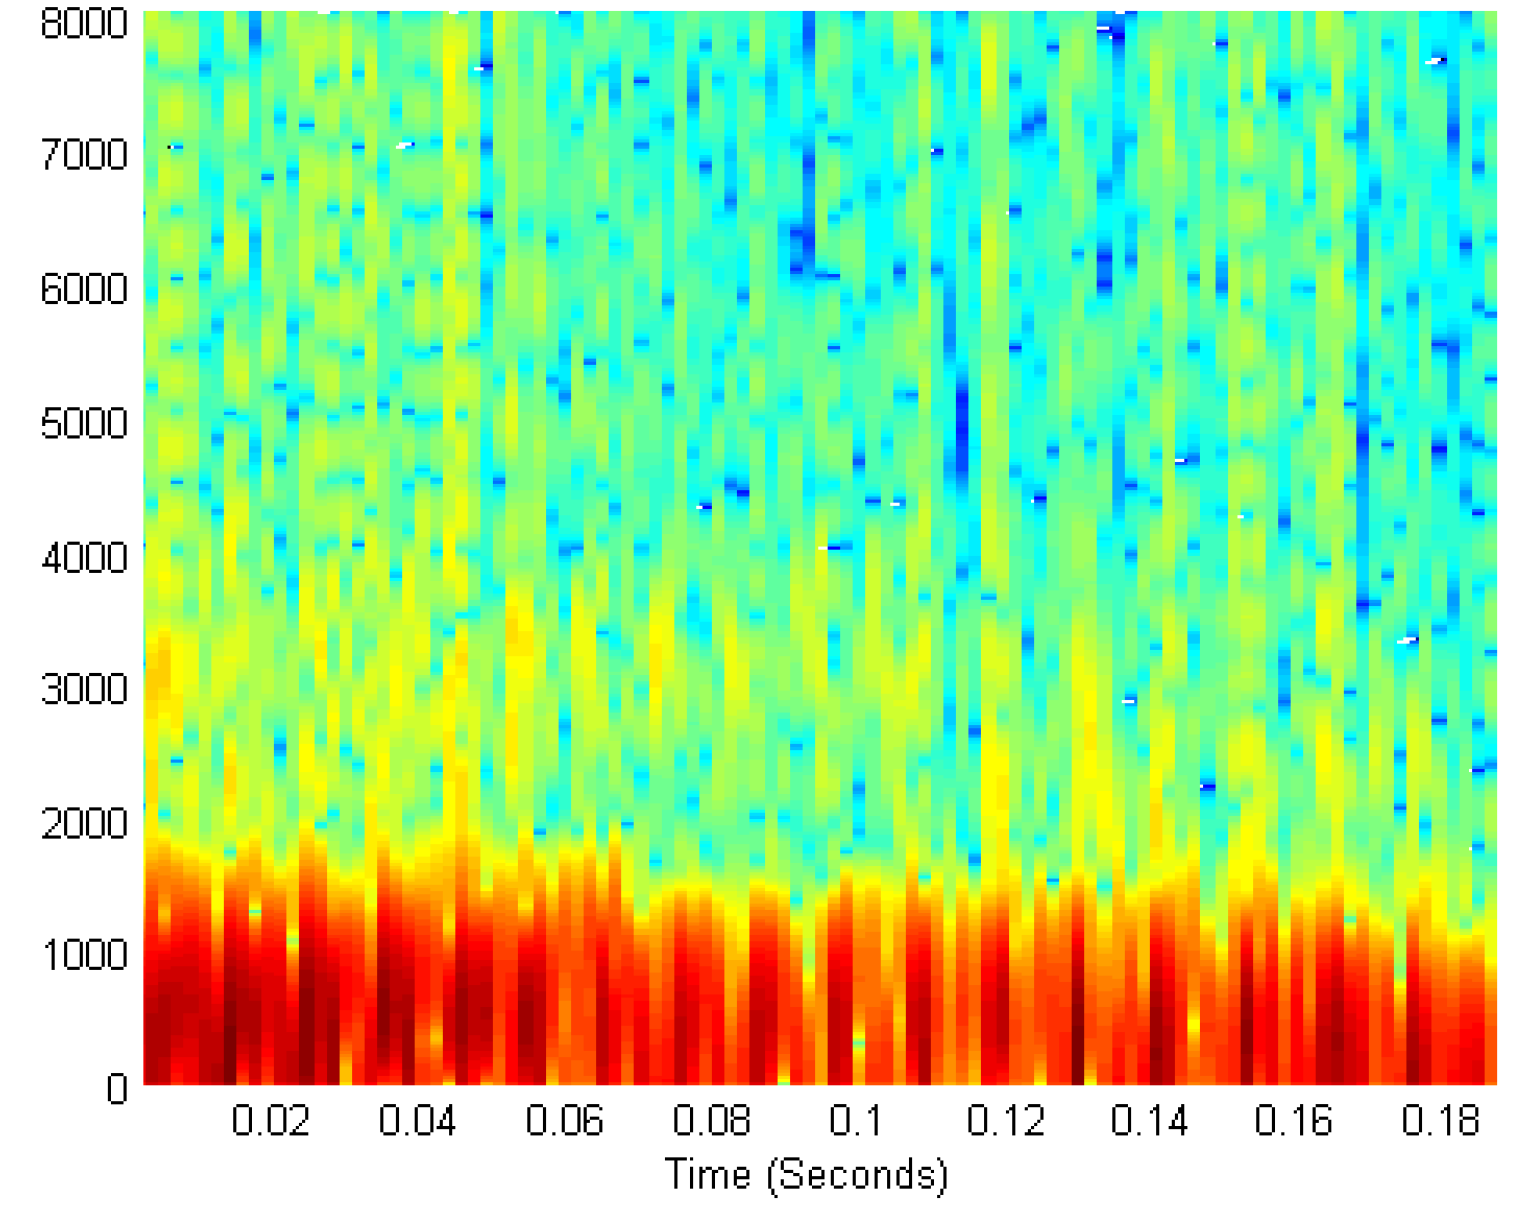
\includegraphics[width=100mm]{TonalRestoratio_Spec_FullRestoration.png}
\begin{picture}(0,0)
\put(-240,235){Spectrogram of signal after full restoration}
\end{picture}
\caption{Example spectrogram of full restoration of audio segment.}
\label{fig:TonalRestoratio_Spec_FullRestoration.png}
\end{figure}

\section{Algorithm statement}
Figure~\ref{fig:restorationPP.pdf} shows a diagrammatic representation of the restoration stage of the algorithm. The restoration stage takes, as an input, $\boldsymbol{w}$ the wavelet packet coefficients, $\boldsymbol{i}$ the detection state and the tonal components. The restoration algorithms take as an input the relevant data to be restored as well as the detection state from the detection algorithm. The restored wavelet packet coefficients $\hat{\boldsymbol{w}}$ are passed through the inverse wavelet packet decomposition algorithm (IWPD) to restore the residual waveform before being combined with the restored tonal component to reconstruct the original restored signal $\hat{x}(n)$.

\begin{figure}%restorationPP.pdf
\centering
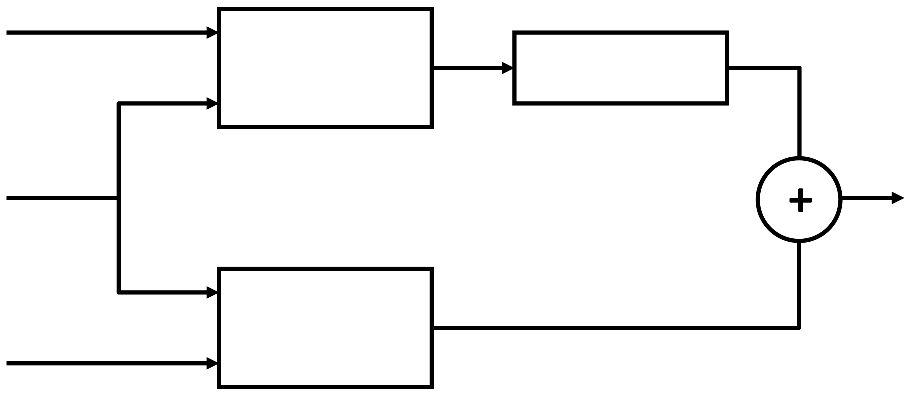
\includegraphics[width=120mm]{restorationPP.pdf}
\begin{picture}(0,0)
%line labels
\put(-330,145){$\boldsymbol{w}$}
\put(-175,130){$\hat{\boldsymbol{w}}$}
\put(-330,80){$\boldsymbol{i}$}
\put(-25,82){$\hat{x}(n)$}
\put(-340,35){Tonal}
\put(-340,20){components}


%box labels
\put(-252,30){Tonal}
\put(-252,15){restoration}
\put(-252,130){Residual}
\put(-252,115){restoration}
\put(-135,120){IWPD}
\end{picture}
\caption{Block diagram showing the general set up of the restoration algorithm.}
\label{fig:restorationPP.pdf}
\end{figure}

\section{Methods}
\subsection{Computational time test}
While most of the results focus on reconstruction quality in various ways, it is important to note that since this algorithm is intended for sequential implementation in communication networks, the computational complexity is of imminent concern. Although traditional complexity measures would rate both the LSAR and the AR filtered algorithms as $O(n^2)$ the actual real world computational time could be vastly different. In an attempt to quantify these differences the code was repeatedly run 1000 times on various machines. The total computational time was divided by the total time for the audio segments processed. While reconstruction was only needed for a fraction of the audio segment length, this scaling gives an average relative computational effort for a real world corrupted signal scenario.

Although non of the code is optimised and the timings are done exclusively in Matlab, the code has been written use Matlab's in-built functions as often as possible. Methods tested all used the same vector segmentation code and so the only differing code was the actual reconstruction process. The computers used for the test were running a variety of Matlab versions but all on the Windows operating system, and all times were conducted using the real time stop watch functions in Matlab. In addition it should be noted that no parallelization, automatic or manual, was enabled within Matlab. Lastly all methods tested were run using the same AR model order and both estimating the AR model solving the Yule-Walker equations.

\subsection{Subjective test}
A subjective listening test was designed to gauge the preference of listeners to reconstructed corruptions in relation to the original corruption. Since the reconstruction procedure, in most cases, still leaves or introduces artifacts in the audio stream the experiment was intended to measure if the artificial noise would in fact be more of an audible nuisance than the original keystrokes.

Subjects were presented with 12 test sets consisting of 2 audio segments each; the original audio segment containing speech and a number of keystrokes and the reconstructed segment. The order of the original segment and the reconstructed segment was randomized throughout the trial. The audio segments used for this test was a mix of fast typing and slow typing, recorded through laptops and external microphones, naturally corrupted segments and keystrokes added to clean segments, male or female speech and a variety of keyboards types and makes.

The Graphical User Interface (GUI) presented to the test subjects is shown here in Figure~\ref{fig:SubjectiveExp_GUI.png}.

\begin{figure}[!] %SubjectiveExp_GUI.png
\centering
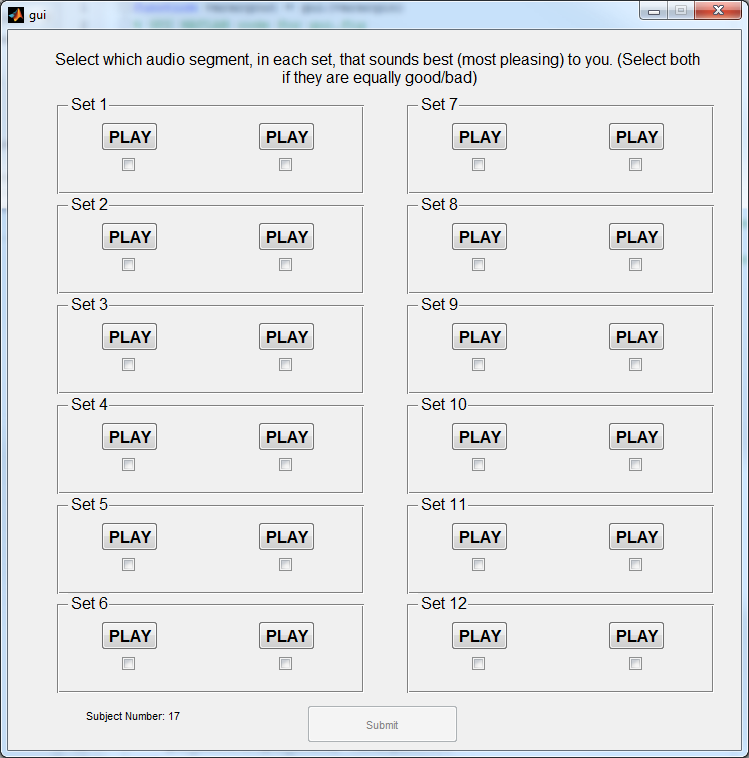
\includegraphics[width=120mm]{SubjectiveExp_GUI.png}
\begin{picture}(0,0)
%\put(-355,120){Frequency}
%\put(-200,0){Time}
\end{picture}
\caption{Experimental GUI presented to subjects.}
\label{fig:SubjectiveExp_GUI.png}
\end{figure}

Subjects were asked to choose their preferred audio segment or the one they found the ``least annoying''. If they found both segments equally annoying or equally pleasing they could opt to tick both boxes and proceed. All audio segments were sampled at 16kHz, ranged from 1 to 10 seconds in length (mainly in the range 3-5 seconds), and were run through a completely sequential version of the final algorithm as it would work implemented in a communication framework. All subjects used the same set of AKG K-240 M1 circumaural open back headphones in a quiet office environment through a laptop computer audio interface and were allowed to replay audio segments as they pleased. The test was conducted on 16 individuals found in and around the office. Most of the subjects were familiar with the research being investigated.

\subsection{Objective tests}
A variety of measures for evaluating the performance and the quality of the reconstructed signals are used as results in this chapter. \todo{more}
\subsubsection{Objective perceptual tests}
The Perceptual Evaluation of Audio Quality (PEAQ) and Perceptual Evaluation of Speech Quality (PESQ) are industry standard perceptual methods for objectively evaluating the perceived quality of audio and speech specifically.

PEAQ is standardized by the International Telecommunication Union's Radiocommunication Sector (ITU-R) through the ITU-R Recommendation BS.1387\cite{BS-1387-1998} of 1998. The implementation used to generate the results in this chapter is the PQevalAudio package from the TSP Lab of McGill University\cite{Kabal2003}. It is noted that ITU-R BS.1387 does not provide sufficient information for a conforming implementation\cite{Campeanu2005} and so PQevalAudio fails to fall within the tight bounds of the standard. Despite this, evaluations of the package does suggest that it comes close enough to warrants its use as a quality impairment measurement\cite{Kabal2003}.

PQevalAudio measures the audio quality with a Mean Opinion Score (MOS) based Objective Difference Grade (ODG) in relation to a reference signal. The MOS\cite{P-800-1996} and Difference grade\cite{Kabal2003} is defined in Table~\ref{tab:MOS} where the description of impairments is the relevant measure for the results in this chapter.

\begin{table}\begin{center}
\caption{Mean Opinion Score (MOS)}
\label{tab:MOS}
\begin{tabular}{|c|c|c|c|}\hline
MOS & Difference Grade  & Quality       & Description of Impairments  \\ \hline
5   & 0                 & Excellent     & Imperceptible               \\
4   & -1                & Good          & Perceptible but not annoying\\
3   & -2                & Fair          & Slightly annoying           \\
2   & -3                & Poor          & Annoying                    \\
1   & -4                & Bad           & Very annoying               \\ \hline
\end{tabular}\end{center}\end{table}

PESQ, or the specific wide band adaptation PESQ-WB\cite{P862-2-2005}, is, unlike PEAQ, designed specifically for speech quality measures, and was first standardised as ITU-Telecommunication (ITU-T) Recommendation P.862 in 2001 with a wide band addition in 2005\cite{P862-2-2005}. The package used to generate the PESQ measures in this chapter was supplied with \cite{Loizou2007}, and quantifies the objective perceptual quality with a MOS of impairments as defined in Table~\ref{tab:MOS}.

It is beyond the scope of this document to further describe the PEAQ and PESQ methods in more detail. Please refer to the cited literature for further detail.

\subsubsection{Other measures}
Further to PEAQ and PESQ, the quality of the reconstructions in this chapter will also be quantified using the Mean Squared Error (MSE). MSE is a measure of the average of the squares of the errors, or the amount which a value differs from a reference value, and is defined by:

\begin{equation}\label{eq:MSEdef}
\textrm{MSE}\left(\hat{x}\right) = \textrm{E} \left[ \left( \hat{x} - x \right)^2\right].
\end{equation}

Here $\hat{x}$ is an estimator and $x$ is the reference value.

A frame based MSE is also used in this chapter to give a temporal representation of the MSE. This measure is simply the MSE applied to overlapping frames throughout the signal.

It is important to stress that the MSE does not give a measure of the perceptibility of an error but just a numeric indication of the magnitude of this error. While a phase shift might be imperceptible to the listener it could potentially give a significant MSE response, while low amplitude noise modulated in phase with a signal could potentially be clearly audible while resulting in only a minor MSE response. For impulsive noise with a large magnitude in relation to the underlying signal it does provide sparse visual reference for evaluating impulsive noise and the reconstruction of corrupted samples and it is to that extent the MSE is primarily used in this chapter.

\todo{Will I even use PSNR?}
The Peak Signal to Noise Ration (PSNR) is a measure of the maximum possible power of a signal in relation to the power of a corrupting noise, and is defined as

\begin{equation}\label{eq:PSNRdef}
\textrm{PSNR} = 20 \log_{10} \left( \frac{\textrm{MAX}_\textrm{I}}{\sqrt{\textrm{MSE}}} \right),
\end{equation}
where MSE\textsubscript{I} is the maximum possible value for a sample.


\section{Results}
\subsection{Preliminary computational measures}
Some benchmark computational results from the reconstruction algorithms are presented in Table~\ref{tab:CompData}. Both methods tested here use an AR model order of 100. In all examples the computational time for the LSAR algorithm is 2 orders of magnitude higher than the simple AR filtering algorithm with noise.

\begin{table}\begin{center}
\caption{Computational time measures relative to audio segment length.}
\label{tab:CompData}
\begin{tabular}{|l|c|c|c|c|c|}\hline
                                % Lenovo            & Home              & Work
                                & PC 1              & PC 2              & PC 3              &  Mean \\ \hline
  Filtering w. noise (wavelet)  & 1.9 $\ttt{-3}$    & 3.4 $\ttt{-3}$    & 2.6 $\ttt{-3}$    &  2.6 $\ttt{-3}$  \\
  Filtering w. noise (waveform) & 1.4 $\ttt{-3}$    & 3.5 $\ttt{-3}$    & 2.4 $\ttt{-3}$    &  2.4 $\ttt{-3}$  \\
  LSAR (wavelet)                & 1.0 $\ttt{-1}$    & 2.3 $\ttt{-1}$    & 2.5 $\ttt{-1}$    &  1.9 $\ttt{-1}$  \\
  LSAR (waveform) (N=100)       & 2.3 $\ttt{0}$     & 0.0 $\ttt{0}$     & 0.0 $\ttt{0}$     &  0.0 $\ttt{0}$  \\ \hline
\end{tabular}\end{center}\end{table}


\subsection{Subjective test}\label{sec:ResultsSubjectiveTest}
% Prefer Recon: 46%, Orig: 36%, Equal: 18%
The results showed that 46\% of the subjects preferred the reconstructed audio segments to the originals, 36\% preferred the original and 18\% were ambivalent and found neither segment better than the other.

Figure~\ref{fig:SubjectiveExp_PerTestData.pdf} shows the results for each of the 12 audio segments. It is clear that subjects generally preferred the reconstructions in sets 5, 10, 11, and 12, where the original was clearly preferred in sets 1, and 2, where the rest of the sets were more mixed in the response. Looking at the sets with a general preference of the reconstructed segment it is noted that these are primarily corrupted by keyboard strokes typed at a slower pace. The slower typed sets also contained fewer keystrokes and it is possible that a higher density of restoration artifacts are more disturbing than keystrokes due to the artifacts' seemingly higher degree of audible variability.

\begin{figure}[!] %SubjectiveExp_PerTestData.pdf
\centering
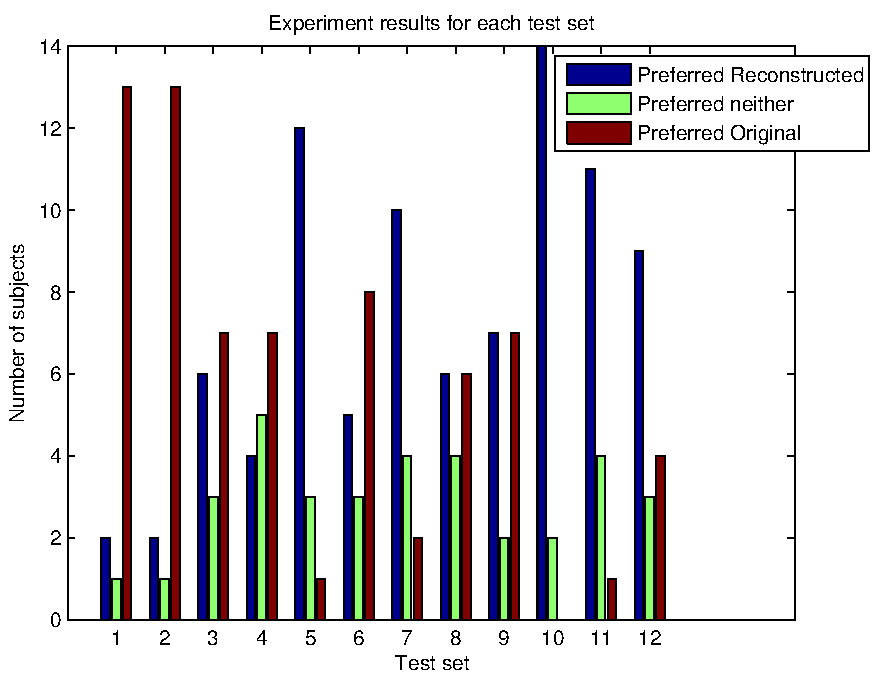
\includegraphics[width=120mm]{SubjectiveExp_PerTestData.pdf}
\begin{picture}(0,0)
%\put(-355,120){Frequency}
%\put(-200,0){Time}
\end{picture}
\caption{Experimental results for each set in the test.}
\label{fig:SubjectiveExp_PerTestData.pdf}
\end{figure}

It was noted that subjects' preferences generally varied greatly. Some subjects almost entirely preferred the original segments while others were heavily in favour of the reconstructions. Most were although split throughout the sets with a slight preference in favour of the reconstructed samples. Figure~\ref{fig:SubjectiveExp_PreferenceHistogram.pdf} shows a histogram of the data from the experiment. From this figure it can be seen how the mode of the distribution of number of preferences of the reconstructed audio segment is higher (7) than that for the number of preference for the original audio segment (4). In other words, 4 subjects preferred the reconstructed segment 7 times in the test, while 4 subjects preferred the original only 4 times.

\begin{figure}[!] %SubjectiveExp_PreferenceHistogram.pdf
\centering
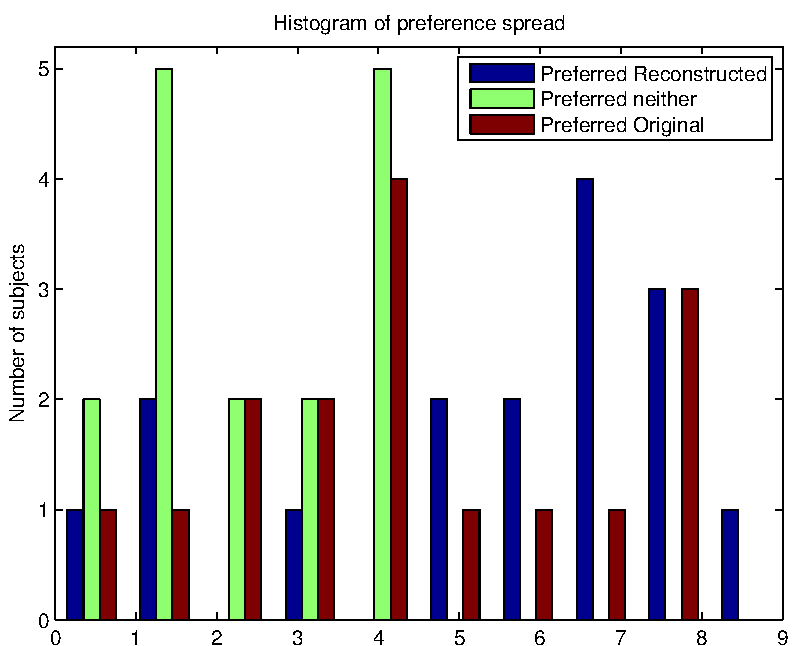
\includegraphics[width=120mm]{SubjectiveExp_PreferenceHistogram.pdf}
\begin{picture}(0,0)
%\put(-355,120){Frequency}
%\put(-200,0){Time}
\end{picture}
\caption{Histogram of test subject preferences.}
\label{fig:SubjectiveExp_PreferenceHistogram.pdf}
\end{figure}

While the results from this test does not conclusively show a preference of the reconstructed audio segments amongst listeners it can be said that there is a slight preference to the reconstructed audio segments. Listeners who were generally in favor of the original segments reported that they preferred the ``naturally'' sounding corruptions to the more artificially soundings corruptions left by the algorithm, especially when these were imbedded in speech. Other users also noted that the key strokes were not generally perceived to be a nuisance at all. These preliminary findings underline the importance of natural and predictably sounding reconstructions.

\subsection{Objective measures}
%should some of that have been in the method section?
The PESQ and the PEAQ test methodologies were used to evaluate some of the data sets used in the subjective test, section~\ref{sec:ResultsSubjectiveTest}, in this chapter. The selected data sets were 2, 4, 6 and 11. Sets 2, 4 and 6 were chosen since, as seen in Figure~\ref{fig:SubjectiveExp_PerTestData.pdf}, the original audio segment was preferred or strongly preferred by the subjects. Set 11 was chosen as a reference for sets were the reconstructed segment was heavily preferred. These sets were also chosen since they were \emph{constructed} segments, meaning that the noisy signal was a linear addition of a clean speech signal and a noise track containing purely keyboard stroke noise. To calculate the PESQ and PEAQ measures, having a reference signal was essential.

Table~\ref{tab:PESQdata} shows the data from the PESQ tests. In all but the set 2 the reconstructed audio sample was found to have a higher MOS, and the mean MOS was found to be 0.2 higher for the reconstructed segments with the biggest improvement being over 0.5 in set 11, which was also the only set which the subjects decidedly preferred the reconstruction over the original segment.

\begin{table}\begin{center}
\caption{PESQ MOS results for test sets 2, 4, 6 and 11.}
\label{tab:PESQdata}
\begin{tabular}{|l|c|c|c|c|c|}\hline
                    & set 2 & set 4 & set 6 & set 11  & Mean \\ \hline
  Reconstruction    & 3.385 & 3.208 & 3.616 & 2.624   & 3.208 \\
  Original          & 3.610 & 2.949 & 3.354 & 2.108   & 3.005 \\ \hline
  Difference        & -0.225& 0.259 & 0.262 & 0.516   & 0.203 \\
  \hline
\end{tabular}\end{center}\end{table}

%Test file: 2
% Prediction for ref3.wav/recon3.wav: PESQ_MOS = 3.385
% Prediction for ref3.wav/dirty3.wav: PESQ_MOS = 3.610

%Test file: 4
% Prediction for ref2.wav/recon2.wav: PESQ_MOS = 3.208
% Prediction for ref2.wav/dirty2.wav: PESQ_MOS = 2.949

%Test file: 6
% Prediction for ref.wav/recon.wav: PESQ_MOS = 3.616
% Prediction for ref.wav/dirty.wav: PESQ_MOS = 3.354

%Test file: 11
% Prediction for ref4.wav/recon4.wav: PESQ_MOS = 2.624
% Prediction for ref4.wav/dirty4.wav: PESQ_MOS = 2.108


Table~\ref{tab:PEAQdataODG} shows the PEAQ ODG MOS for the same audio sets as in Table~\ref{tab:PESQdata}. Again it is seen that the reconstructed audio segments have on average an ODG MOS of 0.4 higher than original signal, with a maximum difference found in the tests conducted on set 6 with a difference of over 1.5 MOS. It was also noted that the preferred segment by the subjects, set 11 reconstructed, was found to have a larger negative difference than the original in contrast to the PESQ results.

\begin{table}\begin{center}
\caption{PEAQ ODG MOS results for test sets 2, 4, 6 and 11.}
\label{tab:PEAQdataODG}
\begin{tabular}{|l|c|c|c|c|c|}\hline
                    % file 3    & file 2    & file 1    & file 4
                    & set 2     & set 4     & set 6     & set 11    & Mean      \\ \hline
  Reconstruction    & -3.678    & -3.599    & -2.066    & -3.889    & -3.308    \\
  Original          & -3.862    & -3.608    & -3.610    & -3.747    & -3.707    \\ \hline
  Difference        & 0.1840    & 0.0090    & 1.5440    & -0.1420   & 0.399     \\
  \hline
\end{tabular}\end{center}\end{table}

The PEAQ implementation used\cite{Loizou2007} featured a couple of other measured that has been included for completeness, including a description of the measures, in section~\ref{ap:PEAQdata} on page~\pageref{ap:PEAQdata}.

\subsection{Other measures}
Table~\ref{tab:MaxMSE} shows the maximum mean squared error (MSE) of collection of sets tested above. It is clearly seen that across the board the reconstructed signal has a lower maximum MSE which is on average 0.3 below the corrupted signal. The set with the most improved max MSE, set 11, and the sets with the least improvement, sets 2 and 4, are also the sets with the strongest polarisation in preference to the same effect of the chosen sets.

\begin{table}\begin{center}
\caption{Max MSE results for test sets 2, 4, 6 and 11.}
\label{tab:MaxMSE}
\begin{tabular}{|l|c|c|c|c|c|}\hline
                    % file 3    & file 2    & file 1    & file 4
                    & set 2     & set 4     & set 6     & set 11    & Mean      \\ \hline
  Reconstruction    & 0.7071    & 0.2052    & 0.2298    & 0.2654    & 0.3519    \\
  Original          & 0.8463    & 0.3739    & 0.6171    & 0.6707    & 0.6270    \\ \hline
  Difference        & -0.1392   & -0.1687   & -0.3873   & -0.4053   & -0.2751    \\
  \hline
\end{tabular}\end{center}\end{table}

An example of one of the frame based MSE comparisons are shown in Figure~\ref{fig:MSEexampleSet11.pdf}. This figure shows a series of corruptions with the a large part of them being detected and restored and as a result exhibit a much reduced MSE. A couple of the noise pulses are not detected and as a result the MSE for both the corrupted signal and the reconstructed signal are identical and overlapping.

\begin{figure} %MSEexampleSet11.pdf
\centering
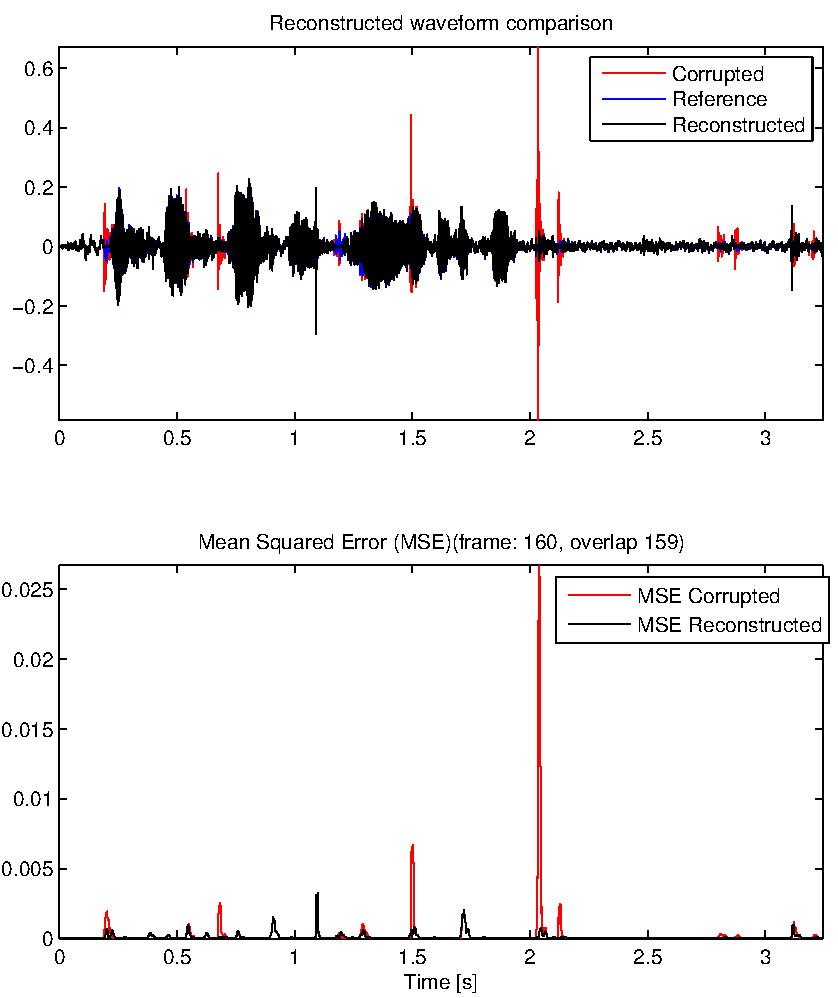
\includegraphics[width=120mm]{MSEexampleSet11.pdf}
\begin{picture}(0,0)
\put(-320,395){(a)}
\put(-320,185){(b)}
\end{picture}
\caption{MSE comparison for data set 11. (a) Corrupted, reconstructed and reference signals, and (b) framed MSE comparison of corrupted and reconstructed signal.}
\label{fig:MSEexampleSet11.pdf}
\end{figure}

Figure~\ref{fig:MSEexampleSet11Zoom.pdf} shows a zoomed in version of Figure~\ref{fig:MSEexampleSet11.pdf} focusing on two major corruptions and one missed detection. The figure shows clearly how the reconstruction algorithm dramatically reduces the MSE of three of the corruptions and almost completely removes the error for one of them. It is also noted that one corruption was not detected and hence no reconstruction was attempted.

\begin{figure} %MSEexampleSet11Zoom.pdf
\centering
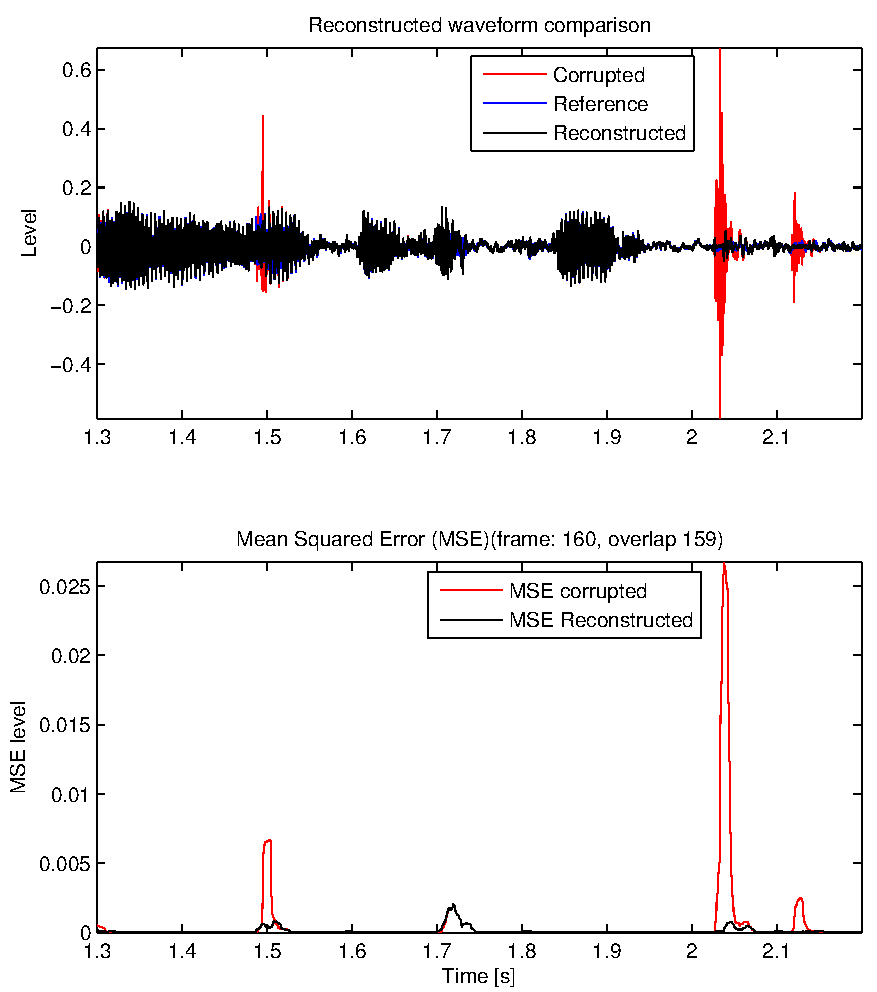
\includegraphics[width=120mm]{MSEexampleSet11Zoom.pdf}
\begin{picture}(0,0)
\put(-320,395){(a)}
\put(-320,185){(b)}
\end{picture}
\caption{Zoomed MSE comparison for data set 11. (a) Corrupted, reconstructed and reference signals, and (b) framed MSE comparison of corrupted and reconstructed signal.}
\label{fig:MSEexampleSet11Zoom.pdf}
\end{figure}

The final measure explored for the 4 selected sets is the peak SNR. Table~\ref{tab:PeakSNR} shows the results from an investigation of the peak SNR calculations. As with the max MSE measures, and to a certain extent the other measures investigated, there appears to be a correlation between the subjective results and the peak SNR measures, with sets 2 and 3 showing less of an improvement than sets 6 and 11. In this case the reconstruction has a peak SNR similar to the original corrupted signal, showing no measurable improvement. In fact the peak SNR is slightly lower for the reconstruction suggesting a deterioration of the signal. On the other hand it is noted that the numbers for sets 6 and 11 are 5.4 and 3.2 dB higher respectively, giving an over all peak SNR of 1.9 dB for the 4 sets.

\begin{table}\begin{center}
\caption{Peak SNR results for test sets 2, 4, 6 and 11.}
\label{tab:PeakSNR}
\begin{tabular}{|l|c|c|c|c|c|}\hline
                    % file 3    & file 2    & file 1    & file 4
                    & set 2     & set 4     & set 6     & set 11    & Mean      \\ \hline
  Reconstruction    & 29.5 dB   & 40.3 dB   & 38.9 dB   & 40.7 dB   & 37.4 dB   \\
  Original          & 30.4 dB   & 40.6 dB   & 33.5 dB   & 37.6 dB   & 35.5 dB   \\ \hline
  Difference        & 5.4 dB    & -0.3 dB   & 0.9  dB   & 3.1  dB   & 1.8  dB   \\
  \hline
\end{tabular}\end{center}\end{table}

\subsection{Waveforms of reconstructions}
\todo{do text}

\begin{figure}%ResultsScaledCombinedExample.pdf
\centering
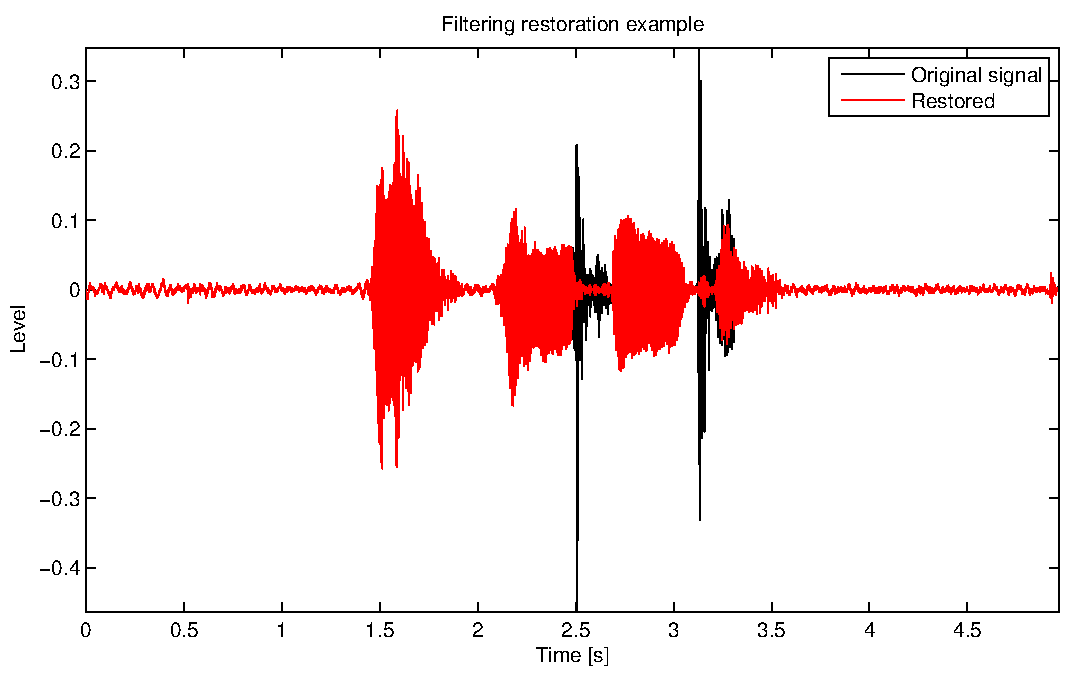
\includegraphics[width=100mm]{ResultsScaledCombinedExample.pdf}
\begin{picture}(0,0)
%\put(-245,235){Restored Wavelet coefficients Example 1}
%\put(-200,0){Time}
\end{picture}
\caption{Time series example of the burst scaling algorithm.}
\label{fig:ResultsScaledCombinedExample.pdf}
\end{figure}


\begin{figure}%RestoredLSARExampleWaveform.pdf
\centering
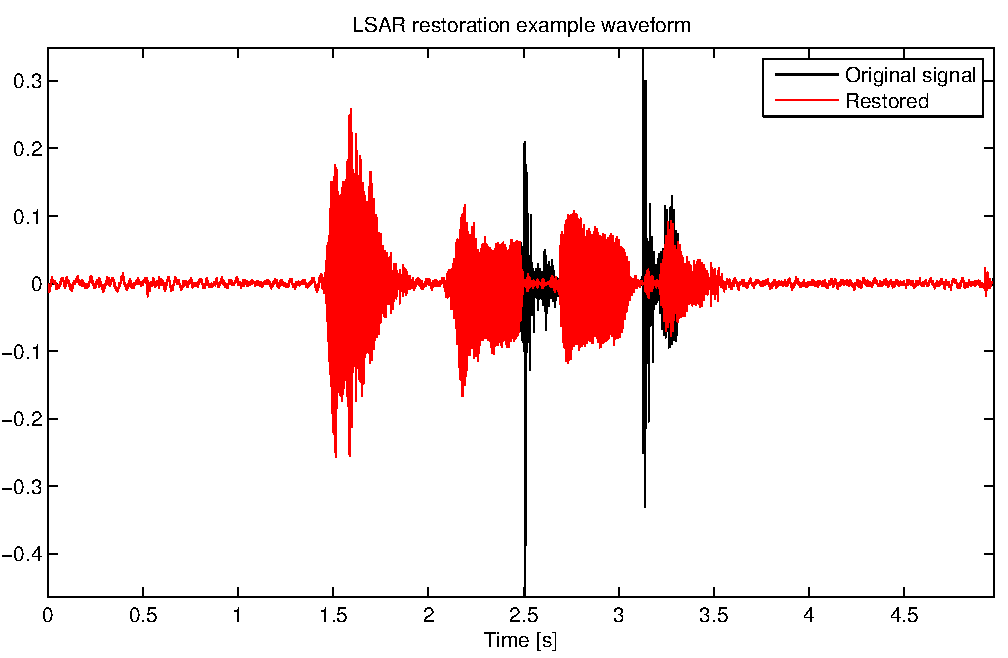
\includegraphics[width=100mm]{RestoredLSARExampleWaveform.pdf}
\begin{picture}(0,0)
%\put(-245,235){Restored Wavelet coefficients Example 1}
%\put(-200,0){Time}
\end{picture}
\caption{Time series example of the LSAR algorithm.}
\label{fig:RestoredLSARExampleWaveform.pdf}
\end{figure}


\section{Discussion}


% Justify the use of a tonal restorer and the specific restorer used


% FIR filtering, computational advantage in the AR parameter estimation
While applying the FIR filtering approaches to the interpolation task for the corrupted samples in the time or the wavelet generated nearly visually and audibly identical results, it is noted that there are some computational advantages to doing it in the wavelet domain. A commonly used approach for estimating the AR parameters is through solving of the Yule-Walker equations. Typical implementations of this algorithm utilise Levison-Durbin recursion which means that the estimation process runs in $\Theta(n^2)$\cite{Hayes1996} rather than $\Theta(n^3)$ using the state of the art Cramer\'s rule implementation\cite{Habgood2012}. Performing the restoration on the wavelet coefficients rather than the waveform will not formally reduce the complexity of the algorithm but for the quadratic complexity recursion the complexity will be reduced by a constant of proportionality since the wavelet packet coefficients will be sampled at $\frac{1}{2^L}$ of the original signal in $2^L$ sets, for a wavelet decomposition at level $L$.

% Justify the use of the AR filtering (filtering with noise) restoration algorithm
Based on the extent of the corruptions, as seen in section~\ref{sec:WPdata}, the residual restoration algorithm's ability to reconstruct longer stretches of missing data is essential. With keyboard strokes affecting upwards of a third of a second, many frames may end up retaining artifacts from the keyboard stroke. The ability of a restoration algorithm to filter or interpolate backwards in a sequential scenario with long corruptions and short frame sizes, is negligible when a simple fading operation can mitigate discontinuities.

%note that tonal noise (especially low frequency bumps) might not be a big nuisance. Possibly due to them not overlapping in spectrum with speech.

\section{Conclusions}

% ------------------------------------------------------------------------


%%% Local Variables:
%%% mode: latex
%%% TeX-master: "../thesis"
%%% End: 